%%%%%%%%%%%%%%%%%%%%%%%%%%%%%%%%%%%%%%%%%
% Oliver Lemon made minor edits (jan 2015)  to :
% Masters/Doctoral Thesis
% LaTeX Template
% Version 1.43 (17/5/14)
%
% This template has been downloaded from:
% http://www.LaTeXTemplates.com
%
% Original authors:
% Steven Gunn
% http://users.ecs.soton.ac.uk/srg/softwaretools/document/templates/
% and
% Sunil Patel
% http://www.sunilpatel.co.uk/thesis-template/
%
% License:
% CC BY-NC-SA 3.0 (http://creativecommons.org/licenses/by-nc-sa/3.0/)
%
% Note:
% Make sure to edit document variables in the Thesis.cls file
%
%%%%%%%%%%%%%%%%%%%%%%%%%%%%%%%%%%%%%%%%%

%----------------------------------------------------------------------------------------
%	PACKAGES AND OTHER DOCUMENT CONFIGURATIONS
%----------------------------------------------------------------------------------------

\documentclass[11pt, oneside]{Thesis} % The default font size and one-sided printing (no margin offsets)

\graphicspath{{Pictures/}} % Specifies the directory where pictures are stored

\usepackage{amsmath}
%\usepackage[square, comma, sort&compress]{natbib} % Use the natbib reference package - read up on this to edit the reference style; if you want text (e.g. Smith et al., 2012) for the in-text references (instead of numbers), remove 'numbers'
\hypersetup{urlcolor=blue, colorlinks=true} % Colors hyperlinks in blue - change to black if annoying

\title{\ttitle} % BUT you should use use " \title{\ttitle} " here instead to define the thesis title !
% \ttitle is defined in the file Thesis.cls

\hyphenation{pro-blem} % Fix hyphenation issues for some words

\begin{document}

\frontmatter % Use roman page numbering style (i, ii, iii, iv...) for the pre-content pages

\setstretch{1.3} % Line spacing of 1.3

% Define the page headers using the FancyHdr package and set up for one-sided printing
\fancyhead{} % Clears all page headers and footers
\rhead{\thepage} % Sets the right side header to show the page number
\lhead{} % Clears the left side page header

\pagestyle{fancy} % Finally, use the "fancy" page style to implement the FancyHdr headers

\newcommand{\HRule}{\rule{\linewidth}{0.5mm}} % New command to make the lines in the title page

% PDF meta-data
\hypersetup{pdftitle={\ttitle}}
\hypersetup{pdfsubject=\subjectname}
\hypersetup{pdfauthor=\authornames}
\hypersetup{pdfkeywords=\keywordnames}

%----------------------------------------------------------------------------------------
%	TITLE PAGE
%----------------------------------------------------------------------------------------

\begin{titlepage}
\begin{center}

\textsc{\LARGE \univname}\\[1.5cm] % University name
\textsc{\Large Masters Thesis}\\[0.5cm] % Thesis type

\HRule \\[0.4cm] % Horizontal line
{\huge \bfseries \ttitle}\\[0.4cm] % Thesis title
\HRule \\[1.5cm] % Horizontal line

\begin{minipage}{0.4\textwidth}
\begin{flushleft} \large
\emph{Author:}\\
\authornames
\end{flushleft}
\end{minipage}
\begin{minipage}{0.4\textwidth}
\begin{flushright} \large
\emph{Supervisors:} \\
\supname
\end{flushright}
\end{minipage}\\[3cm]

\large \textit{A thesis submitted in fulfilment of the requirements\\ for the degree of \degreename}\\[0.3cm] % University requirement text
\textit{in the}\\[0.4cm]
%\groupname\\

\deptname\\[2cm] % Research group name and department name

{\large \today}\\[1cm] % Date
\includegraphics[width=6cm]{./Figures/HWUlogo.jpg} % University/department logo - uncomment to place it

\vfill
\end{center}

\end{titlepage}

%----------------------------------------------------------------------------------------
%	DECLARATION PAGE
%	Your institution may give you a different text to place here
%----------------------------------------------------------------------------------------

\Declaration{

\addtocontents{toc}{\vspace{1em}} % Add a gap in the Contents, for aesthetics

I, \authornames, declare that this thesis titled, \guille{\ttitle} and the work presented in it is my own. I confirm that this work submitted for assessment is my own and is expressed in my own words. Any uses made within it of the works of other authors in any form (e.g., ideas, equations, figures, text, tables, programs) are properly acknowledged at any point of their use. A list of the references employed is included.

%\begin{itemize}
%\item[\tiny{$\blacksquare$}] This work was done wholly or mainly while in candidature for a research degree at this University.
%\item[\tiny{$\blacksquare$}] Where any part of this thesis has previously been submitted for a degree or any other qualification at %this University or any other institution, this has been clearly stated.
%\item[\tiny{$\blacksquare$}] Where I have consulted the published work of others, this is always clearly attributed.
%\item[\tiny{$\blacksquare$}] Where I have quoted from the work of others, the source is always given. With the exception of such %quotations, this thesis is entirely my own work.
%\item[\tiny{$\blacksquare$}] I have acknowledged all main sources of help.
%\item[\tiny{$\blacksquare$}] Where the thesis is based on work done by myself jointly with others, I have made clear exactly what %was done by others and what I have contributed myself.\\
%\end{itemize}
\vspace{2cm}
\textbf{Signed}: \includegraphics[width=5cm]{./Figures/Signature.png}\\
\rule[1em]{25em}{0.5pt} % This prints a line for the signature

\textbf{Date}: 24th of July, 2020 \\
\rule[1em]{25em}{0.5pt} % This prints a line to write the date
}

\clearpage % Start a new page

%----------------------------------------------------------------------------------------
%	ABSTRACT PAGE
%----------------------------------------------------------------------------------------

\addtotoc{Abstract} % Add the "Abstract" page entry to the Contents

%\abstract{\addtocontents{toc}{\vspace{1em}} % Add a gap in the Contents, for aesthetics

 {\huge{\textit{Abstract}} \par}{\addtocontents{toc}{\vspace{1em}}

Computers can represent numbers in different ways. Representations of them can differ in their binary translation. Integers, Floating-Point and Fixed-Point representations coexist with their own benefits and drawbacks. Reduced- and mixed- precision have been a focus of the literature since the 1960's. Using lower precision often increases performance at the cost of negligible loss in accuracy. The application are extremely diverse and growing emphasis is noticeable around machine learning and artificial intelligence. While training neural networks may require a powerful setup, deploying a network in an application should be possible on low-power, low-resource hardware architecture. Reconfigurable architectures have proven to be more powerful and flexible than GPUs when looking at a specific application. This thesis aims to assess the impact of mixed-precision when applied to a neural network deployed on reconfigurable hardware. While several frameworks have been developed to create tools to deploy neural network using reduced-precision, few benchmarks have been set up to assess the importance of quantisation and the quality of the benchmark. The benchmark set up here is used on top of \emph{FINN} and \emph{Brevitas}, two frameworks from Xilinx labs. While the results correspond to the intuition for neural networks using 2 to 16 bits for their parameters, networks using 32 bits precision seem to outperform the others both in terms of throughput and accuracy.
%The page is kept centered vertically so can expand into the blank space above the title too\ldots
%


\clearpage % Start a new page

%----------------------------------------------------------------------------------------
%	ACKNOWLEDGEMENTS
%----------------------------------------------------------------------------------------

\setstretch{1.3} % Reset the line-spacing to 1.3 for body text (if it has changed)

\acknowledgements{\addtocontents{toc}{\vspace{1em}} % Add a gap in the Contents, for aesthetics

My thanks go to every person that helped during the redaction of this paper. I am grateful for Pr. Loïc Lagadec and Dr. Pascal Cotret that proposed the subject to me. I thank them for their weekly guidance and help. I also want to express my gratitude for Pr. Rob Stewart that accepted to supervise the project as well. He helped ensure the report was resourceful and on point with the aimed project.

My thanks also go to the developers in the Xilinx Research Labs that provided me with a board to conduct my experiments on and guided me in a lot of steps through the development of their tools. My thanks go to M. Yaman Umuroglu, M. Alessandro Pappalardo and M. Henrik Borras for their insight and quality advice.
}
\clearpage % Start a new page

%----------------------------------------------------------------------------------------
%	LIST OF CONTENTS/FIGURES/TABLES PAGES
%----------------------------------------------------------------------------------------

\pagestyle{fancy} % The page style headers have been "empty" all this time, now use the "fancy" headers as defined before to bring them back

\lhead{\emph{Contents}} % Set the left side page header to "Contents"
\tableofcontents % Write out the Table of Contents

\lhead{\emph{List of Figures}} % Set the left side page header to "List of Figures"
\listoffigures % Write out the List of Figures

\lhead{\emph{List of Tables}} % Set the left side page header to "List of Tables"
\listoftables % Write out the List of Tables

%----------------------------------------------------------------------------------------
%	ABBREVIATIONS
%----------------------------------------------------------------------------------------

\clearpage % Start a new page

\setstretch{1.5} % Set the line spacing to 1.5, this makes the following tables easier to read

\lhead{\emph{Abbreviations}} % Set the left side page header to "Abbreviations"
\listofsymbols{ll} % Include a list of Abbreviations (a table of two columns)
{
\textbf{MNIST}    & \textbf{M}odified \textbf{N}ational \textbf{I}nstitute of \textbf{S}tandard and \textbf{T}echnology \\
\textbf{CIFAR-10} & \textbf{C}anadian \textbf{I}nstitute \textbf{F}or \textbf{A}dvanced \textbf{R}esearch 10            \\
\textbf{SVHN}     & \textbf{S}treet \textbf{V}iew \textbf{H}ouse \textbf{N}umbers                                       \\
\textbf{GTSRB}    & \textbf{G}erman \textbf{T}rafic \textbf{S}ign \textbf{R}ecognition \textbf{B}enchmark               \\

\textbf{FC Layer} & \textbf{F}ully-\textbf{C}onnected Layer                 \\
\textbf{NN}       & \textbf{N}eural \textbf{N}etwork                        \\
\textbf{CNN}      & \textbf{C}onvolutional \textbf{N}eural \textbf{N}etwork \\
\textbf{QNN}      & \textbf{Q}uantised \textbf{N}eural \textbf{N}etwork     \\
\textbf{BNN}      & \textbf{B}inarised \textbf{N}eural \textbf{N}etwork     \\

\textbf{GPU}      & \textbf{G}raphics \textbf{P}rocessing \textbf{U}nit                          \\
\textbf{CUDA}     & \textbf{C}ompute \textbf{U}nified \textbf{D}evice \textbf{A}rchitecture      \\
\textbf{MPI}      & \textbf{M}essage \textbf{P}assing \textbf{I}nterface                         \\
\textbf{NCCL}     & \textbf{N}vidia \textbf{C}ollective \textbf{C}ommunications \textbf{L}ibrary \\
\textbf{ASIC}     & \textbf{A}pplication \textbf{S}pecific \textbf{I}ntegrated \textbf{C}ircuit  \\

\textbf{FPGA}     & \textbf{F}ield \textbf{P}rogrammable \textbf{G}ate \textbf{A}rray \\
\textbf{HLS}      & \textbf{H}igh \textbf{L}evel \textbf{S}ynthesis                   \\
\textbf{LUT}      & \textbf{L}ook-\textbf{U}p \textbf{T}able                          \\
\textbf{FF}       & \textbf{F}lip-\textbf{F}lop                                       \\
\textbf{BRAM}     & \textbf{B}lock \textbf{R}andom \textbf{A}ccess \textbf{M}emory    \\
\textbf{DRAM}     & \textbf{D}ynamic \textbf{R}andom \textbf{A}ccess \textbf{M}emory  \\
\textbf{DSP}      & \textbf{D}igital \textbf{S}ignal \textbf{P}rocessor               \\

\textbf{I/O}      & \textbf{I}nput / \textbf{O}utput                       \\
\textbf{SVG}      & \textbf{S}tochastic \textbf{G}radient \textbf{D}escent \\
}

%----------------------------------------------------------------------------------------
%	THESIS CONTENT - CHAPTERS
%----------------------------------------------------------------------------------------

\mainmatter % Begin numeric (1,2,3...) page numbering

\pagestyle{fancy} % Return the page headers back to the "fancy" style

% Include the chapters of the thesis as separate files from the Chapters folder
% Uncomment the lines as you write the chapters

\chapter{Introduction}\label{chap_intro} % Main chapter title

\label{Chapter1} % For referencing this chapter elsewhere, use \ref{Chapter1}

\lhead{Chapter 1. \emph{Introduction}}

%----------------------------------------------------------------------------------------
%	SECTION 1.1 - Context
%----------------------------------------------------------------------------------------

\section{Context}

Ever since the creation of computers, their computation power has been a source of progress in terms of high-precision scientific computations in one hand or efficient energy expensive mass computations. In one case or the other, this performance has been met through the development of more and more performant hardware architectures. Moore forecasted the evolution through his law announced in 1965. However, the last decade has proven to counterbalance this law and makes it meet an end due to physical and thermal limitations. This decrease in hardware evolution has rather shifted the focus to other vectors of performance. One of them is parallelisation through the use of multiple or a cluster of computers. The goal is then to increase the computational power. This focus has enabled the development of new architectures tailored to those specific tasks, such as Graphical Processing Units (GPUs) or reprogrammable architectures such as Field Programmable Gate Arrays (FPGAs). In parallel, the use of reduced precision to increase the performance of computational-expensive tasks is a focus of the literature that can be applied particularly well to state-of-the-art hardware architectures. Next chapters look over the ideas under mixed-precision and the ways to implement them efficiently. Next derive applications that can benefit from the implementations and their translation to physical architectures.

%-----------------------------------
%	SECTION 1.2 - Aims and Objectives
%-----------------------------------
\section{Aims and Objectives}

The aim of the thesis is to give the reader an insight of the mixed-precision mindset and intentions by covering important articles and ideas the literature holds. The practical aim and result of the literature review is to implement a specific application using mixed-precision. This application consists of deploying a \emph{quantised neural network} (i.e. a neural network using reduced-precision) on a \emph{reconfigurable architecture}.

The resulting aims are the following. The objectives will be defined after the literature review in the \guille{Requirements analysis} chapter.

\textbf{Aims}
\begin{enumerate}
  \item Provide the reader with notions in \emph{Number Representation}.
  \item Provide the reader with notions in \emph{Machine Learning}.
  \item Provide the reader with notions in \emph{Hardware Architecture}.
  \item Link the three pools of notions through the \emph{Literature Review}.
  \item Present the objective of the project: Deploy a \emph{neural network} on a \emph{reconfigurable architecture}.
  \item Present the mixed-precision \emph{motivations} and \emph{implementation methods}.
  \item Present the mixed-precision \emph{applications} to machine learning.
  \item Present the \emph{frameworks} and \emph{deployment solutions} for machine learning on reconfigurable architectures.
  \item Present an \emph{implementation of a benchmark} over a framework.
  \item Display \emph{results of the benchmarking}.
  \item Provide the reader with \emph{critics} on the results.
  \item Give out possible \emph{future works} or applications.
\end{enumerate}

%-----------------------------------
%	SECTION 1.3 - Structure of the report
%-----------------------------------

\section{Structure of the report}

The given thesis is structured as follows. \textbf{Chapter 1} provides a brief \emph{Introduction} to the context and objectives of the report. \textbf{Chapter 2} consists of the \emph{Background}, presenting the main ideas behind both \emph{number representation}, \emph{machine learning} and \emph{hardware architectures}. \textbf{Chapter 3} covers the \emph{Literature Review} and how \emph{mixed-precision} was implemented and used, how it can be applied to \emph{neural networks} and how \emph{neural networks} can be deployed on specific architectures. \textbf{Chapter 4} consists of a \emph{Requirement Analysis} of the development project of the dissertation. \textbf{Chapter 5} presents any \emph{Professional, Legal, Ethical and Social Issues} the project can highlight. \textbf{Chapter 6} consists of a presentation of the implementation of the project, it goes over the main points and presents the tools and frameworks used as well as the experiments performed. \textbf{Chapter 7} presents the results of the experiments while \textbf{Chapter 8} discusses the results and leads to future works that can extend the project. Finally, \textbf{Chapter 9} is the \emph{Conclusion} of the thesis.

\chapter{Background} % Main chapter title

\label{Chapter2} % For referencing this chapter elsewhere, use \ref{Chapter2}

\lhead{Chapter 2. \emph{Background}}

%----------------------------------------------------------------------------------------
%	SECTION 2.1 - Background - Number representation
%----------------------------------------------------------------------------------------

\section{Background: On Number Representation}

The question of the representation of numbers as we, humans, use them in a world of electronics has been central in the creation of computers and their associated arithmetics. Several problems are contained in the simple question of: How to translate our arithmetic and number operations in a piece of hardware?

%-----------------------------------
%	SUBSECTION 2.1.1 - Number Representation
%-----------------------------------
\subsection{Number Representation}

The first thing to note is that electronics can represent two states, a presence or absence of an electric impulsion. The states of \guille{on} and \guille{off} is embedded in transistors that can represent both. The transistor is the hardware representant of this duality while a bit is its software counter-part. This is the underlying reason why computers, even the first fully electronical computer ENIAC (\emph{Electronical Numerical Integrator and Computer}), use a binary system. If this system is handy to translate our base 10 arithmetic and simple numbers such as integers, it is harder to translate more complex numbers such as reals and floating point operations. The meaning of an N-bit binary word is entirely dependent of the interpretation we choose to use. This interpretation consists of both a representation (the type of the object the memory represents) and its associated mapping. Common number representations consists of unsigned integers, signed integers (using two's complement), floating point reals as well as fixed-point reals.

%-----------------------------------
%	SUBSUBSECTION 2.1.1.1 - Integer Representation
%-----------------------------------
\subsubsection{Integer Representation}

The representation of integers and especially unsigned integers is straightforward as it consists of a change form base 10 to base 2. This number representation can be done in 16-bits, 32-bits or 64-bits depending on its type, the supporting hardware and the space we need to contain it. Representing a number in base 2 from base 10 or vice versa is straightforward as it only demands simple and exact basic operations to be performed. As shown on \emph{Figure} \ref{fig:IntegerRepr}, $4576 = 2^5 + 2^6 + 2^7 + 2^8 + 2^12$.

Now, if we want to represent a signed integer, we have to use a method called the \emph{two's complement} in order to bring the sign in. This method keeps the basic behaviour of the addition to work on numbers be they positive or negative. The method consists in changing the value of all the bits of a given number then adding one to the result. The representation of -4576 when doing the computation with 13 bits (1 sign bit and 12 mantissa bits) consists of:

\begin{align}
(01000111100000)^\text{two's complement} &= (01000111100000)^\text{one's complement} + 1
                                           &= 10111000011111 + 1
                                           &= 10111000100000
\end{align}

The result for 32 and 64 bits can be seen on \emph{Figure} \ref{fig:IntegerRepr}.

\begin{figure}[htbp]
	\centering
		\includegraphics[width=.8\textwidth]{Figures/IntegerRepr.png}
	\caption[Integer Representation]{Integer Representation and Two's Complement example}
	\label{fig:IntegerRepr}
\end{figure}

Those two representations allow a complete mapping of integers up to a certain range: signed 32-bit integers can represent base 10 numbers between -2,147,483,648 and 2,147,483,647 while unsigned integers can represent base 10 numbers between 0 and 4,294,967,295.

%-----------------------------------
%	SUBSUBSECTION 2.1.1.2 - Floating-Point Representation
%-----------------------------------
\subsubsection{Floating-Point Representation}

Representing floating-point numbers has been a concern since the 1980's and the industrial development of several computing modules and interfaces. The need for a consensus in this domain and particular applications has been answered by the IEEE-754 standard \cite{Ieee754_1985} in 1985. This standard defines both the floating-point number representations and exceptions conditions along with their default handling. This norm was reviewed fundamentally in 2008 \cite{Ieee754_2008}, extending it to 64-bits and 128-bits length. The last dated revision of the norm is from 2019 \cite{Ieee754_2019}.

Floating-point numbers following this representation are composed of three distinct elements:
\begin{enumerate}
  \item A sign bit
  \item An exponent
  \item A mantissa
\end{enumerate}

Those three elements compose the number by using the following formula: $(\mathit{sign}) \times \mathit{mantissa} \times 2^{\mathit{exponent}}$

In order to present both positive and negative exponents and as using the two's complement on the exponent would complexify the computation of floating-point numbers, a bias is used in the exponent. This bias corresponds to $2^e - 1$ where e is the number of bits of the exponent part. This means that with an 8-bit exponent, the bias is equal to 127. An exponent equal to $00000111$ is equal to $7 - 127 = -120$ and an exponent equal to $10000111$ is equal to $135 - 127 = 8$. An 8-bit exponent can cover a range from -126 to 127 (because exponents -127 (all 0s) and +128 (all 1s) are reserved for special numbers.

When referring to single-precision floating-point representation we are talking about 32-bit long memory representation. They are mapped as follows and as shown in \emph{Figure} \ref{fig:FP32}:
\begin{itemize}
  \item Sign bit: 1 bit
  \item Exponent: 8 bits
  \item Mantissa: 23 bits
  \item Exponent Bias: 127
\end{itemize}

% FP32 EXAMPLE
\begin{figure}[htbp]
	\centering
		\includegraphics[width=.8\textwidth]{Figures/FP32.png}
	\caption[Single-precision float representation]{Example of the representation of a float in single-precision}
	\label{fig:FP32}
\end{figure}

Referring to double precision floating-point representation means looking at 64-bit long memory representation, mapped as follows and as shown in \emph{Figure} \ref{fig:FP64}:
\begin{itemize}
  \item Sign bit: 1 bit
  \item Exponent: 11 bits
  \item Mantissa: 52 bits
  \item Exponent Bias: 127
\end{itemize}

% FP64 EXAMPLE
\begin{figure}[htbp]
	\centering
		\includegraphics[width=.8\textwidth]{Figures/FP64.png}
	\caption[Double-precision float representation]{Example of the representation of a float in double-precision}
	\label{fig:FP64}
\end{figure}

Along these representations, IEEE-754 introduces representations of special numbers. Positive and negative infinities are encoded with all 1s exponents and a fraction equal to zero. Zero is encoded with an all-0s exponent and fraction. Moreover, it adds methods to round floating-point numbers to positive or negative infinity, zero or to the nearest value.

%-----------------------------------
%	SUBSUBSECTION 2.1.1.3 - Fixed-Point Representation
%-----------------------------------
\subsubsection{Fixed-Point Representation}

Another way to look at the decimals is to fix the radix point to be at a certain place and keep it throughout all the computations and representations using this arithmetic. A fixed-point representation consists of three components:
\begin{enumerate}
  \item A sign indicator
  \item An integer corresponding to the total number of bits
  \item Another integer corresponding to the size of the fractional part
\end{enumerate}

Representing a number with this representation can be done by simply concatenating the base 2 representation of each side of the radix point. This means the integer part will be represented with positive powers of two ($2^0$,$2^1$,$2^2$,...) while the fractional part is represented with negative powers of two ($2^{-1}$, $2^{-2}$,...).

% FIXED POINT EXAMPLE
\begin{figure}[htbp]
	\centering
		\includegraphics[width=.8\textwidth]{Figures/FixedPoint.png}
	\caption[Fixed-Point Representation]{Example of a float in fixed-point representation}
	\label{fig:FixedPoint}
\end{figure}

As shown in \emph{Figure} \ref{fig:FixedPoint}, several representations can depict the same decimal number. Finding the correct amount of bits to allocate to each side of the radix point is what will qualify the representation. Allocating fewer bits than needed may lead to overflow while allocating too much may increase quantisation errors.
Along with this new representation comes a whole new arithmetic. While this format can help tailor your needs in terms of variable types, it comes with an additional cost. The operations performed in this arithmetic are non-trivial as addition and multiplication are not associative and distributive anymore. This means the order of the operations will have an impact on the final result. Moreover, the round-off error underlying this representation is often non-trivial to grasp. However, those operations are low demanding in terms of computing power.

%-----------------------------------
%	SUBSECTION 2.1.2 - Performance Benchmarks
%-----------------------------------
\subsection{Metrics \& Performance benchmarks}

Floating-point representation (in either single or double precision) allows extreme precision at the cost of performance trade-offs (space or memory). On the other hand, fixed-point representation, even if it comes with a more complex arithmetic and insidious round-off errors, allows to tailor the type to your needs. Storing the values of the size and mass of planets in floating-point precision, would end up not using the majority of the range of values you selected while one could tailor a correct type in fixed-point representation.

The benchmarks in this field use several metrics in order to quantify and qualify the representations and their implementations.
\begin{itemize}
	\item \textbf{Size}: The size of a number in a given representation.
	\item \textbf{Energy cost}: The cost of operations in a given representation. \emph{The lower the better}.
	\item \textbf{Frequency}: The clock rate of a piece of hardware, or the quickness of pulses generation. \emph{The lower the better}.
	\item \textbf{Latency}: The access time of a piece of hardware to memory or external devices. \emph{The lower the better}.
	\item \textbf{Accuracy}: The precision enabled by a given representation. \emph{The higher the better}.
	\item \textbf{Memory Usage}: The memory needed to store both numbers and results of operations between them. \emph{The lower the better}.
	\item \textbf{Performance}: The overall time needed to complete a sequence of operations.
\end{itemize}

The operations performed in floating-point are expensive in terms of bandwidth, memory and energy consumption, which ultimately translate in to additional cost to perform an action. Horowitz's talk at ISSCC 2014 \cite{Horowitz2014} entitled \guille{Computing's Energy Problem (and what we can do about it)} provides an insight of the problems and challenges technology scaling has encountered in its development. Moore's law is getting outdated and a solution to the issue of permanently growing energy needs resides in \guille{the design of applications and hardware that are better matched to task and each other}. The numbers presented by M.Horrowitz have been reused by Professor William Dally (Standford University, NVidia Corporation) in his lecture on \guille{High-Performance Hardware for Machine Learning} \cite{Nips2015}. The \emph{Figure} \ref{fig:OpCosts} is extracted from this lecture and presents the energy and area costs different floating-point operations demand. Increasing precision on the used numbers increases the relative energy cost at the same time. An 8-bit addition costs 0.03 pJ whereas the same addition in 32-bit floating-point costs 0.9 pJ or 30 times more.

% COSTS OF OPERATIONS 2015-NIPS
\begin{figure}[htbp]
	\centering
		\includegraphics[width=\textwidth]{Figures/OpCosts.png}
	\caption[Operation costs]{Cost of operations in certain representations \cite{Nips2015,Horowitz2014}}
	\label{fig:OpCosts}
\end{figure}

The benefit of using a more optimised representation other the floating-point representation has been investigated as soon as in 2000 in \cite{Tong2000}. The authors present a way to reduce the energy consumption by minimising the bitwidth representation of the floating-point data. The data used to tailor the type representation is human-sensory data such as speech or video imagery. This kind of data is obtained at low precision (4 to 10 bits) but mapped into a full single-precision floating-point type. Using such optimisations, the authors manage to obtain a reduction of 66\% in multiplier energy per operation without sacrificing any accuracy.

Modifications of the representations can be embedded in the architecture. Xilinx, a manufacturer of state-of-the-art architecture, produced a white paper written by Finnerty et al. \cite{Xilinx2017} showing that their tools are able to handle fixed-point types and arithmetic and that the benefits are important:
\begin{itemize}
  \item Reduced power consumption
  \item Reduced use of resources (look-up tables, memory)
  \item Latency improvements
  \item Comparable performance and accuracy
\end{itemize}
The authors show the example of an FIR filter implementation in fixed-point representation from floating-point. The frequency is shown to be 16\% faster and the latency 7.5 times lower.

In conclusion, customising type in an environment where costs are translated in terms of energy consumption, memory or bandwidth usage, will always come out as an improvement. This redirects the issue to a need to guarantee little to no loss in accuracy.

%----------------------------------------------------------------------------------------
%	SECTION 2.2 - Background - Machine Learning
%----------------------------------------------------------------------------------------

\section{Background: On Machine Learning}

Machine Learning is one of the most promising asset of the recent years since it has proven to be reliable when tackling complex issues. Those tasks can either be recognizing a street sign, a disease in a radiography or classifying a piece of text under a sentiment. Text-to-speech, speech-to-text, image classification, object detection, etc. Those are all thedomains machine learning is suited for. This section will provide insight on the basic functions machine learning uses, present neural network architectures and development frameworks.

%-----------------------------------------------
%	SUBSECTION 2.2.1 - Neurons and Neural Networks
%-----------------------------------------------

\subsection{Neural Networks}

 Machine learning has been extended to the use of neural networks. Karpathy et al. \cite{Karpathy2015} present the different structures in their lecture materials. The apparition of neural networks in machine learning comes from the analogy with the human brain and the way neurons work and communicate between each other. The analogy can be seen on \emph{Figure} \ref{fig:Neuron}.

% NEURON PRESENTATION
\begin{figure}[htbp]
	\centering
		\includegraphics[width=8cm]{Figures/Neuron.png}
	\caption[Neuron Example]{Example of a neuron and its behavior in a neural network \cite{Karpathy2015}}
	\label{fig:Neuron}
\end{figure}

Each neuron receives several inputs from other previous neurons and performs an operation on all the received inputs to create the output that will go to its successors. A family of neurons that will obtain the outputs of the same neurons is called a \emph{layer}. A combination of \emph{layers} composes a \emph{neural network} as presented on \emph{Figure} \ref{fig:NN}.

% NEURAL NETWORK PRESENTATION
\begin{figure}[htbp]
	\centering
		\includegraphics[width=8cm]{Figures/NN.png}
	\caption[Neural Network Example]{Example of a neural network architecture \cite{Karpathy2015}}
	\label{fig:NN}
\end{figure}

The neuron performs a simple dot product of all the inputs along with their weights, adds a bias to the sum and applies a given non-linear activation function. The weight will give importance to some of the inputs while hiding others. Throughout the training, some of the inputs will be shown to be more useful than others and their weight will be changed accordingly. The function used by the neuron (dot-product here) depends on the type of the layer the neuron is part of.The activation function models the \guille{firing rate of the neuron which [...] represents the frequency of the spikes along the axoms}. It is often a simple non-linear function that will help a network have an answer against non-linear problems. The XOR function for example can be learned by a network composed of as little as two layers. Several choices of non-linear functions can be made for your neurons:
\begin{itemize}
  \item Sigmoid function: $\sigma(x) = \frac{1}{(1+e^{-x})}$
  \item Tanh: $tanh(x) = 2\sigma(2x) - 1$
  \item Rectified Linear Unit (ReLU): $ f(x) = max(0,x) $
\end{itemize}

Neural networks perform the simple operations of reducing the inputs, adding a bias and passing it through a non-linear function. However, it is possible to set up several layers where the first one is called the \emph{input layer}, the last one the \emph{output layer} and all the layers in-between the \emph{hidden layers}. These layers go one after each other as shown in \emph{Figure} \ref{fig:NN}. While having hidden neurons is useful to better comprehend the data fed to the network, having too much of them can lead to overfitting, including noise and outliers into the pattern recognition.

Neural networks perform well in machine learning, but the fields where the architecture is mostly used are image and speech recognition. An extension of neural networks is used when the data is known to be of a certain type. For example, if the data is known to be images, Convolutional Neural Networks (CNN) are the best choice as they are tailored with the goal of handling images. They are a special type of neural networks in the sense that they use 3D layers and transformations on images. This choice of 3D layers comes from the fact that images are usually encoded in three channels, RGB (Red, Green and Blue). CNNs can be used for image classification, object detection, image segmentation or speech recognition. We will focus on image recognition here as this field provides well-known metrics and network layouts due to the popularity of the ImageNet Project for example \cite{ImageNet2009}. This popularity has attracted literature focus and allows comparisons and benchmarks to be made.

% NEURAL NETWORK PRESENTATION
\begin{figure}[htbp]
	\centering
		\includegraphics[width=8cm]{Figures/CNN.png}
	\caption[Convolutional Neural Network Example]{Example of a convolutional neural network architecture \cite{Karpathy2015}}
	\label{fig:CNN}
\end{figure}

Several layers are used and allow to perform different operations on images. The most used and well-known are the following:
\begin{itemize}
  \item Convolution   (CONV): Connects small regions of the input image through a filter. \emph{This layer helps extracting features such as edges or shapes.}
  \item Activation     (ACT): Apply an activation function (such as $max(0,x)$). \emph{This layer brings non-linearity into place.}
  \item Pooling       (POOL): Downsampling operation through a filter. \emph{This layer replaces a region of the image with the max or average value. It helps reducing noise.}
  \item Fully-Connected (FC): Computation of the class scores. \emph{This layer consists of a reduce operation and allows to compute the class scores.}
\end{itemize}

Layers take as input a set of data, known as a \emph{Feature Map} and output a new set of feature maps with higher-level semantics. Those layers then compose a CNN architecture and can be trained on a bank of images to adjust the different bias and weights for each layers and their corresponding neurons. Finally, once the network is trained, it can deduce the class of a given image. Those two steps are called \emph{Training} and \emph{Inference}, the training will work on a set of annotated data samples to create a model \guille{which semantics extrapolate outside the training set, [with a] \emph{modelling power}} \cite{Abdelouahab2018}. Once this step is completed, the \emph{Inference} phase can start and the network will have to classify new data instances. The training phase is extremely consuming in terms of time, energy and hardware resources. However, it only needs to be performed once. On the other hand, the inference has to be run each time a new instance is provided to the system. Therefore, if literature focus on accelerating both phases, an emphasis is put on inference as it will be needed to embark trained networks in lighter architectures.

%-------------------------------------------------
%	SUBSECTION 2.2.2 - Tools for Classification
%-------------------------------------------------

\subsection{Tools for Classification}

%-----------------------------------------------
%	SUBSUBSECTION 2.2.2.1 - Network Architectures
%-----------------------------------------------

\subsubsection{Network Architectures}

While there exists a wide range of applications for neural networks and machine learning in general, the field of image classification is the most suitable to benchmarking. Literature presents a wide and evergrowing number of neural networks, often backed up by reknowned companies. Historically, Yann LE CUN et al. \cite{LeCun} presented the first version of a CNN tailored to a specific task: recognizing handwritten digits. By the same occasion, they created the MNIST (Modified National Institute of Standards and Technology) dataset to benchmark their network architecture. All CNN architectures are composed of two main phases:
\begin{itemize}
  \item \emph{Feature Extraction}: This phase consists of an extraction of features by downsampling the image through several filter layers (convolutions, pooling but also batch normalisation and dropout).
  \item \emph{Classification}: This phase consists of flattening the output of the first phase and running it through several linear layers with varying number of neurons. The final linear layer will always have a number of neurons equal to the number of classes in the classification challenge.
\end{itemize}

Le Cun et al. \cite{LeCun1998} architecture chose to tackle the two phases by designing a neural network architecture called \emph{LeNet}. This architecture represents the feature extraction phase by using a succession of two $5 \times 5$ convolutions and $2 \times 2$ average pooling layers. Then, three linear layers (fully connected) perform the classification. Their respective size are 120, 84 and 10 (the number of classes in MNIST \cite{LeCun2010} case which it was designed for). The activation function used is hyperbolic tangent. This whole architecture is displayed on \emph{Figure} \ref{fig:LeNet-5} representing the version \emph{LeNet-5}.

% LeNet-5 PRESENTATION
\begin{figure}[htbp]
	\centering
		\includegraphics[width=8cm]{Figures/LeNet-5.png}
	\caption[LeNet-5]{Architecture of LeNet-5 as taken from \cite{LeCun1998}}
	\label{fig:LeNet-5}
\end{figure}

Krizhevsky et al. present \emph{AlexNet} \cite{Krizhevsky2012} in 2012, 14 years later, as the succesor of \emph{LeNet}. \emph{AlexNet} consists of deeper and wider version of \emph{LeNet}. There are now five convolution layers (of respective filter size $11 \times 11$, $5 \times 5$ and $3 \times 3$ for the remaining). Maximum pooling is used instead of average and it is the first time the ReLU function is used as an activation function ($max(0,x)$ as a reminder). The three final layers are now sized as 4096, 4096 and 1000 (the number of classes of the ImageNet \cite{ImageNet2009} dataset). This whole architecture is displayed on \emph{Figure} \ref{fig:AlexNet}.

% AlexNet PRESENTATION
\begin{figure}[htbp]
	\centering
		\includegraphics[width=8cm]{Figures/AlexNet.png}
	\caption[AlexNet]{Architecture of AlexNet as taken from \cite{Krizhevsky2012}}
	\label{fig:AlexNet}
\end{figure}


Using the same idea that Krizhevsky et al. \cite{Krizhevsky2012} had in mind when designing \emph{AlexNet} in 2014, Simonyan et al. took it a step further when designing \emph{VGGNet} \cite{Simonyan2014}. The VGG net comes with different versions (11, 13, 16 and 19) corresponding to the number of convolutions and fully-connected layers. Using only $3 \times 3$ convolution filters and the same size of linear layers, VGG-16 performed very well on ImageNet \cite{ImageNet2009}. Its architecture is displayed on \emph{Figure} \ref{fig:VGG-16}. One of the downside of this very-deep neural network is that it holds an enormous amount of parameters taking memory space. VGG-16 for example takes about 500MB of memory.

% VGG-16 PRESENTATION
\begin{figure}[htbp]
	\centering
		\includegraphics[width=8cm]{Figures/VGG-16.png}
	\caption[VGG-16]{Architecture of VGG-16 as taken from \cite{Simonyan2014}}
	\label{fig:VGG-16}
\end{figure}

From now on, extending the layer size and network depth does not seem to give better results. Reknowned companies are now enrolling in the battle to the best accuracy on the ImageNet dataset \cite{ImageNet2009} and Microsoft presents its \emph{ResNet} \cite{He2015} in the 2015 competition. \emph{ResNet} uses a method to add a way to skip some connections. During the training of a network, all weights receive an update proportional to the gradient. If this gradient is very small, the change in weight can be minimal and the network can stop its training. Microsoft Research used those skipping connections to conserve the signal and mitigate data loss. In other words, \emph{ResNet} breaks a deep neural network into smaller networks connected through skip or shortcut connections. Its architecture is displayed on \emph{Figure} \ref{fig:ResNet-50}.

% ResNet-50 PRESENTATION
\begin{figure}[htbp]
	\centering
		\includegraphics[width=8cm]{Figures/ResNet-50.png}
	\caption[ResNet-50]{Architecture of ResNet-50 as taken from \cite{He2015}}
	\label{fig:ResNet-50}
\end{figure}

Google came into place by proposing the \emph{MobileNet} \cite{Howard2017} architecture. This architecture, as its name shows, aims at being embarked in many mobile or light hardware architectures. Its emphasis is put on the size of the network and should allow the developer to tailor it to the needs of his aimed hardware architecture. The number of parameters is reduced by using a \guille{\emph{separable depthwise convolution}} that separates the usual $3 \times 3$ convolution into two parts. The first one applies the filter on the inputs and the second (a $1 \times 1$ filter called \guille{\emph{pointwise convolution}}) combine the outputs. Overall, this technique allows to reduce the number of parameters and operations while keeping state-of-the-art.

% % MobileNet PRESENTATION
% \begin{figure}[htbp]
% 	\centering
% 		\includegraphics[width=8cm]{Figures/MobileNet.png}
% 	\caption[MobileNet]{Architecture of MobileNet as taken from \cite{He2015}}
% 	\label{fig:MobileNet}
% \end{figure}

Many other networks exist and are still being developed actively. New techniques (e.g. batch normalisation \cite{Ioffe2015}) are getting incorporated in state-of-the-art architectures to get an even better result out of them. This list is in no way exhaustive but presents the milestones and wishes to translate the mindset operating in the machine learning community.

% TODO Table simplifying the different networks -> number of parameters, year, methodology, etc.

%----------------------------------
%	SUBSUBSECTION 2.2.2.2 - Datasets
%----------------------------------

\subsubsection{Datasets}

The architectures presented earlier are well-known and are still getting better with version iterations and the discovery of new techniques (batch normalisation, depth-wise convolution, residuals, etc.). On the other side, datasets have evolved to present each time a new and harder challenge for different architectures to perform on. Well-known datasets consist of the following:
\begin{itemize}
  \item \emph{MNIST} is the historical dataset, considered as the machine learning version of a classic \guille{\emph{hello world}}. It was implemented along with the \emph{LeNet} architecture and has been the default first dataset to train a network architecture on ever since. Several extensions to this dataset have been created since the dataset is juged to be \guille{too easy} to be a challenge to modern neuron architectures. Very simple CNN can achieve less than 3\% error on this dataset. Several drop-in replacements have been developed such as \emph{Fashion-MNIST} \cite{Xiao2017} - set up by Zalando with simple images of garnments -, \emph{Kuzushiji-MNIST} \cite{Clanuwat2018} - three versions on the recognition of Japanese characters - or even \emph{MNIST-MIX} \cite{Jiang2020} - a mix of handwritten digits from different languages -. All the instances of the MNIST dataset and its variations are images with only one channel (grey levels) and sized 28 pixels by 28 pixels. Those images are labelled in 10 different classes (digits from 0 to 9).

  % MNIST PRESENTATION
  \begin{figure}[htbp]
  	\centering
  		\includegraphics[width=8cm]{Figures/MNIST.png}
  	\caption[MNIST]{Instances extracted from the MNIST dataset}
  	\label{fig:MNIST}
  \end{figure}

  \item \emph{CIFAR-10} are labelled subset from the \emph{Tiny Images} dataset \cite{Krizhevsky2009}. It has been created in 2009 as collected and labelled automatically, supervised by three researchers from the MIT. This dataset is composed of tiny ($32 \times 32$) colored (3 channels) images of ten different classes: airplane, automobile, bird, cat, deer, dog, frog, horse, ship and truck. Instances taken from this dataset can be seen on \emph{Figure} \ref{fig:CIFAR-10} A more complicated dataset has been created in the same way. It is called \emph{CIFAR-100}, and as its name might suggest, contains a hundred different classes.

  % CIFAR-10 PRESENTATION
  \begin{figure}[htbp]
  	\centering
  		\includegraphics[width=8cm]{Figures/CIFAR-10.png}
  	\caption[CIFAR-10]{Instances extracted from the CIFAR-10 dataset}
  	\label{fig:CIFAR-10}
  \end{figure}

  \item With a growing emphasis put on autonomous vehicles, datasets have been developed accordingly. The two most well-known datasets covering this area are \emph{SVHN} (Street View House Numbers) \cite{Netzer2011} and \emph{GTSRB} (German Traffic Sign Recognition Benchmark) \cite{Stallkamp2012}. These two datasets have colored images of variable dimensions. \emph{SVHN} is an extension of \emph{MNIST} in the sense that it is a combination of different digits that the network will have to recognize. On the other hand, \emph{GTSRB} has been used in a 2012 competition and is useful to prototype self-driving components. \emph{GTSRB} contains 43 different classes of colored images and an instance of each of them can be seen on \emph{Figure} \ref{fig:GTSRB}.

  % % SVHN PRESENTATION
  % \begin{figure}[htbp]
  % 	\centering
  % 		\includegraphics[width=8cm]{Figures/SVHN.png}
  % 	\caption[SVHN]{Instances extracted from the SVHN dataset}
  % 	\label{fig:SVHN}
  % \end{figure}

  % GTSRB PRESENTATION
  \begin{figure}[htbp]
  	\centering
  		\includegraphics[width=8cm]{Figures/GTSRB.png}
  	\caption[GTSRB]{Instances extracted from the GTSRB dataset}
  	\label{fig:GTSRB}
  \end{figure}

  \item Finally, \emph{ImageNet} \cite{ImageNet2009} is one of the largest dataset developed. It has been put up by a team from the Princeton University and is the centre of a challenge each year where state-of-the-art architectures confront themselves to get the best accuracy possible. The challenge is named the ImageNet Large Scale Visual Recognition Challenge (ILSVRC). Every year, contesters try to get the best possible accuracy out of the network they propose. The images contained in the dataset are $224 \times 224$ colored images split in 20,000 classes. The dataset contains more than 14 million images and has become the benchmark to determine the accuracy and robustness of state-of-the-art architectures.

  % IMAGENET PRESENTATION
  \begin{figure}[htbp]
  	\centering
  		\includegraphics[width=8cm]{Figures/ImageNet.png}
  	\caption[ImageNet]{Instances extracted from the ImageNet dataset}
  	\label{fig:ImageNet}
  \end{figure}

\end{itemize}

% TODO: INCLUDE Table simplifying the different datasets

%-----------------------------------------------------
%	SUBSUBSECTION 2.2.2.3 - Development Frameworks
%-----------------------------------------------------

\subsubsection{Development Frameworks}

As research in the field of machine learning keeps growing and attracting more and more focus, many different development frameworks emerged to propose a high-level API and environment to experimental needs. Major industrial actors used this opportunity to present their own development API. Each one of the leading companies in IT has its own version of AI environment. Most of them have been under development for nearly a decade and still continue to attract a growing audience.

\begin{itemize}
  \item \emph{Tensorflow} has been the initiative of Google in 2011 and its source code has been opened in 2015. It is, to this day, the most used development framework in the field of machine learning. Its API is designed for Python and C\+\+. However, due to increasing attention, numerous bindings to other languages have been created (Java, C\#, Haskell, etc.). Tensorflow set the milestones for AI frameworks by implementing production-ready resource distribution to deploy one's network to anyy architecture (CPU, GPU or a cluster). It also implements the idea of a \emph{tensor}, a ditributed array.
  \item Microsoft launched in 2015 its \emph{Cognitive Toolkit (CNTK)} written in C++ that aims at the same objectives as \emph{Tensorflow}: easy network creation through a high-level API and simplified deployment to a variety of architectures.
  \item The first version of \emph{Caffe (Convolutional Architecture for Fast Feature Embedding)} was developed in the University of Berkeley in 2014. In 2017, Facebook used \emph{Caffe} in an extended version called \emph{Caffe2} and as of May 2018, \emph{Caffe2} is officially merged in the \emph{PyTorch} project.
  \emph{Torch} is a Lua-based framework that was created in 2002. It is not in active development anymore since 2018 but \emph{PyTorch}, a Python implementation of the same underlying logic is in active development with a specific focus on the research community. \emph{Pytorch} aims at rapid prototyping and flexible architectures.
\end{itemize}

In the end, chosing a framework depends on one's objectives and knowledge of the language used. Benchmarks are getting released with, for example, Luo et al. \cite{Luo2020} that present a mobile implementation of several network architectures (\emph{ResNet, Inception, DenseNet, etc.}) implemented in \emph{TensorFlow Lite, Caffe2 and PyTorch Mobile}. The benchmark the authors propose is named \emph{AIoTBench} and focuses on computer vision. Few other initiatives have been published. The choice is purely personal for now.

% TODO: INCLUDE Table comparing the different development frameworks

%----------------------------------------------------------------------------------------
%	SECTION 2.3 - Background Hardware Architecture
%----------------------------------------------------------------------------------------

\section{Background: On Hardware Architecture}

Moore's law \cite{Moore2006} predicted the evolution of hardware capacities in years to come when defined in 1965. It is an empirical relationship and in no means a physical or natural law but has shown to be exact for the thirty years following its creation. The Moore's law, when announced in 1965 said that \guille{the number of components per integrated circuit would double every year}. This law held for a decade and was then revised to \guille{doubling every two years} for the next decade. This law has been an industry guideline and helped produce long term business plans. However, the law is slowly coming to an end and has been shown to not fulfill the prophecy anymore due to physical limitations such as thermal restrictions. New architectures will have to take the lead as more computational power is still needed for the years to come. What are the new ways and architectures to increase performance even more?

%-----------------------------------
%	SUBSECTION 2.3.1 - GPU
%-----------------------------------

\subsection{GPU}

One solution to enable hardware acceleration is to parallelise computationally expensive tasks. GPUs (\emph{Graphics Processing Units}) are specialised electronic circuits that can handle computationally demanding tasks such as 3D rendering, video encoding and decoding or any action that can be massively parallelised (cryptocurrency digging, matrix computations or brute-force cracking). Few companies actually conceive and sell such systems. The most famous are NVidia, AMD and Intel and some smaller fabless - conceive the circuit but integrally subcontract the production -  companies such as Qualcomm or ARM. Other manufacturing companies such as ASUS or MSI will then integrate those circuits into products and calibrate them along with a cooling system that can make it enhance its base abilities.

Along with GPUs come their proper Software Development Kit (SDK) in order for developers to use their tools. NVidia invested heavily in CUDA (\emph{Compute Unified Device Architecture}) \cite{CUDA} and its aim is to reproduce a C syntax and environment for GPUs. AMD and Intel provide open-source SDK that tools then built upon.

GPUs allow computers to delegate expensive tasks (3D rendering for example) from the CPU to them. The GPUs can be either integrated or external. They require less knowledge than FPGAs but provide a more static architecture that will limit tuning opportunities. Mixed-precision mindset will not reach its full potential with this architecture but will still manage to increase the performance of different operations and tasks.

GPU provide an easy access to parallelisation and allow researchers of different fields to experiment with different precisions and parallelisation. One field that benefits a lot from it is the field of physics and applied simulations. Inherently, mathematics benefit a lot from reduced precisions in terms of computation times and resource utilisation to perform clasic operations such as matrix factorisation. Next are some examples of GPU application in the world of mixed-precision along with the hardware used.

\begin{itemize}
  \item \emph{Mathematics:} Haidar et al. \cite{Haidar2018} present a mixed-precision method to factorise a matrix into two triangular matrices. In order to perform their experiments, they use two 10-cores \emph{Intel Xeon e5-2650 v3} CPUs and one \emph{NVidia V100 PCLe} GPU.
  \item \emph{Mechanical Engineering:} Goddeke et al. \cite{Goddeke2007} present a survey paper on mixed-precision applied to \emph{Finite Element Simulations}, a widely used method in physics simulations that often require extensive computational resources. In their experiments, they use an \emph{AMD Athlon64 X2 4400} CPU and an \emph{NVidia GeForce 7800 GTX} GPU.
  \item \emph{Geosimulation:} Ichimura et al. \cite{Ichimura2018} present a mixed-precision earthquake simulator with an IA designed to help the solver converge. They use several super-computers such as the \emph{Summit} comprising two \emph{IBM Power9} processors and six \emph{NVidia Volta V100 accelerators}.
  \item \emph{Nuclear physics:} Clark et al. \cite{Clark2010} use mixed-precision in their work on simulating the quarks\' interactions in a nucleon. They use an \emph{NVidia GeForce GTX 280} GPU.
\end{itemize}

GPUs represent a fair part of the marketshare due to their various usages. They often come as a cheap and easy access to parallelisation since they have a wide and diverse community with ready-to-go frameworks and implementations.

%-----------------------------------
%	SUBSECTION 2.3.2 - FPGA
%-----------------------------------

\subsection{FPGA}

On the other hand, the 1990's have seen the birth of a new type of architecture: reconfigurable hardware. They allow to create application-specific hardware and are mixed-precision by default. Xilinx, one of the most famous FPGA manufacturer describes them as consisting of \guille{up to two million logic cells that can be configured to implement a variety of software algorithms} \cite{Xilinx2017}. Those logic cells can be dynamically reconfigured and this is the strength of this architecture.

Modern FPGAs contain components that are specilialised for specific functions as well as more general purpose configurable logic. The combination of specific components with the configurable logic has allowed for architectures that consume less power and perform more efficiently.
\begin{itemize}
  \item \emph{Configurable Logic Block (CLB):} A \emph{CLB} is the most basic FPGA component which provide both logic and storage functionalities. It can be anything like a transistor, NAND gate, multiplexor or any combination of these. It often comes with a \emph{Look-Up Table (LUT)} to perform logic operations and a \emph{Flip-Flop (FF)} acting as a register for the results of the \emph{LUT}.
  \item \emph{Digital Signal Processing (DSP) Block:} A \emph{DSP block} is a specialised component of an FPGA that is designed to carry out \emph{digital signal processing} functions such as filtering or multiplying. It is designed to be much more efficient than if it was made with several \emph{CLBs}.
  \item \emph{Transceiver:} A \emph{trans-ceiver} is made to \emph{trans}-mit and re-\emph{ceive} serial data (individual bits) to and from the FPGA at extremely high rates. It also checks for erroneous data in the transmission. Having a dedicated component made it both quicker and easier to communicate with the FPGA.
  \item \emph{Block Random Access Memory (BRAM):} A \emph{BRAM} is the dedicated memory on the chip. This type of block can be divided or cascaded to make smaller or larger memory chunks available.
  \item \emph{Input/Output (I/O) Block}: The \emph{I/O block} operates, as its name gives out, as a component through which data transfers in and out of the FPGA. They are similar to \emph{transceivers} but are more flexible in functionality while operating at slower speed.
\end{itemize}

Along with those base components come many high-end more interesting components that can help develop the hardware to be tightly linked to the application one has in mind. As stated by \cite{Goddeke2007}, FPGAs have native mixed-precision processors and \guille{there is no need to utilise the same number format throughout the algorithm, or even the same operation}. Moreover, the freedom in the number representation can lead to alternative feasible number representations, such as a logarithmic one.

FPGAs can help prototyping chips and perform system validation, including pre-silicon validation, post-silicon validation and firmware development. Manufacturers can therefore validate their design before the chip is produced in factory. The end product can be an ASIC for example, an extremely powerful computing unit that is tailored to one function and one function only. Even though FPGAs are slower than ASICs and consume more power, their inherent ability to be reconfigurable makes them interesting in certain applications. Microsoft uses FPGAs to speed up Bing searches and still be able to change the search algorithm if needed. The efficiency versus flexibility can be seen on \emph{Figure} \ref{fig:EfficiencyVSFlexibility}.

% FPGA/ASIC comparison
\begin{figure}[htbp]
	\centering
		\includegraphics[width=\textwidth]{Figures/EfficiencyVSFlexibility.png}
	\caption[EfficiencyVSFlexibility]{Efficiency vs Flexibility, source: \emph{Bob Broderson, Berkeley Wireless Group}}
	\label{fig:EfficiencyVSFlexibility}
\end{figure}

One downside of FPGAs is the need for intrinsic knowledge of a Hardware Description Language (HDL) or one of their higher-level abstractions \cite{XuanSang2014}. While this step can be a downside, it also brings up a new layer of customisation, tuning and tests. The whole development cycle shown in \emph{Figure} \ref{fig:FPGACycle} can be controlled using a high-level development language such as Smalltalk in \cite{XuanSang2014}. Finer-grain tuning can be performed using the direct HDL language but the learning curve is steeper.

% FPGA Development Cycle
\begin{figure}[htbp]
	\centering
		\includegraphics[width=\textwidth]{Figures/FPGACycle.png}
	\caption[FPGA Development Cycle]{FPGA Development Cycle \cite{XuanSang2014}}
	\label{fig:FPGACycle}
\end{figure}

\chapter{Literature Review} % Main chapter title

\label{Chapter3} % For referencing this chapter elsewhere, use \ref{Chapter2}

\lhead{Chapter 3. \emph{Literature Review}}

%----------------------------------------------------------------------------------------
%	SECTION 3.1 - Mixed Precision
%----------------------------------------------------------------------------------------

\section{Mixed Precision}

The first section explained in details the different existing number representations. With a particular emphasis on the representation of floating-point number, it has shown what the underlying issues of such representations are. The question now is how can we use to our advantage the different types along with their strengths and weaknesses?

%-----------------------------------
%	SUBSECTION 3.1.1 - Motivations
%-----------------------------------
\subsection{Motivations}

The term \guille{mixed precision} comes from the idea of using different precisions (type representations) to increase the performance of a computation that would otherwise only use the highest available (or user-defined) precision. The previous section showed us that each number representation has its pros and cons. Using lower precision types and representations will allow the total computation to decrease the usage of several hardware resources (memory, bandwidth, energy consumption) \cite{Horowitz2014,Nips2015}.

However, if lower-precision is acceptable, using mixed-precision can increase the capacity of smaller systems and subsystems as it will increase the overall performance and resources usage. This goal is targeted when you are aiming for the most performant processor, being given a size and type of usage. Moreover, this can be used when you know exactly the tasks your system will perform as well as their needed size. Yates \cite{Yates2007} presents several rules allowing  to determine the required size of any operation performed in fixed-point arithmetic. This arithmetic allows to tailor the type size to one's needs. Reconfigurable hardware can take advantage of this as well by using the exact required size for an operation. Such architecture will be looked upon in the next sections.

Scientific computations often require the highest available precision and the reduced precision induced by the lower-precision components is unacceptable. In order to still take advantage of the several gains lower-precision provides, a compromise has to be found about how and when to use lower-precision. Ideas on the usage have been looked upon since the 1950's and the first methods to correctly implement them in the early 1960's.

In any case, the developer has to know and keep in mind:
\begin{itemize}
  \item Required end precision
  \item Acceptable error rate
  \item Actual operations performed by the system
\end{itemize}

Mixed precision methods consist of doing a large part of the computation in low-precision components and only a small part in high-precision. As presented in the survey paper \cite{Goddeke2007} using different formats in the same algorithm can have several beneficial properties such as:
\begin{itemize}
  \item Accuracy: Same accuracy when up to 99\% of the operations is performed in the low format
  \item Computation: Low precision operations require less transistors and can translate in more paralellism
  \item Memory: Reduction in size in memory influences the efficiency and bandwidth requirements positively
\end{itemize}

%-----------------------------------
%	SUBSECTION 3.1.2 - Methods and Implementations
%-----------------------------------

\subsection{Methods and Implementations}
Several methods to actually implement a mixed precision algorithm have been developed starting 60 years ago. If the methods are different in practice, the theory behind them is the same as they aim to delegate most of the work to low-precision components while only using high-precision to recover the desired accuracy for the computation.

%-----------------------------------
%	SUBSUBSECTION 3.1.2.1 - Iterative Refinement
%-----------------------------------

\subsubsection{Iterative Refinement}

Since the early 1960's, literature has studied the effects and ways to implement mixed precision. The first reported works to implement such methods are James H. Wilkinson \cite{Wilkinson1994} and Cleve Moler \cite{Moler1967}. The method presented by both is named \guille{iterative refinement} and uses a combination of accumulative inner products along with a linear solver. This solution is directed towards the resolution of a system in the form of $Ax=b$ for a quadratic $N*N$ matrix $A$. The main idea is to use a residual between the wanted result and the result obtained by the last iteration. This residual is computed using high precision and accumulated using high-precision as well while the resolution of the equation is done in low-precision.

% Iterative Refinement Example
\begin{figure}[htbp]
	\centering
\begin{tabular}{ll}
	$x^{(0)}=0$ &\\
	$d^{(s)}=b-Ax^{(s)}$ & Compute residual in \emph{high} precision\\
	$Ac^{(s)}=d^{(s)}$ & Solve equation system in \emph{low} precision\\
	$x^{(s+1)}=x^{(s)}+c^{(s)}$ & Accumulate solution in \emph{high} precision\\
\end{tabular}
	\caption[Iterative Refinement]{Iterative Refinement Method \cite{Goddeke2007}}
	\label{fig:IterativeRef}
\end{figure}

This method has later been reused and extended. Baboulin et al. \cite{Baboulin2009} combine single- and double-precision floating-point numbers to enhance the performance of \guille{dense and sparse linear algebra algorithms}. Strzodka et al. \cite{Strzodka2006} present an enhanced algorithm to resolve a partial differential equation (Poisson problem) to present the effects of a mixed-precision approach. Sun et al. \cite{Sun2008} reproduce a linear solver in mixed-precision but adds an error analysis. The last two articles implement the result of their research on a reprogrammable architecture. Several applications profit directly from these papers and their implementations of mixed-precision algorithms as seen in later sections.

%-----------------------------------
%	SUBSUBSECTION 3.1.2.2 - Iterative Refinement
%-----------------------------------

\subsubsection{Analysis and Rewriting}

When creating a new application or system, any developer tends to use the highest available (or one of the highest) to represent the numbers he will need. However, the space and operations performed on higher-precision types are, as shown earlier, not the most performant. A simple, yet effective way to choose the correct type is to analyse the code and rewrite types that can be represented by lower precision ones. This idea has been implemented in the code analysis tool Precimonious \cite{Rubio2013} for floating-point representations. This analysis tool can go over the code and determines parts of it where lower precision can apply.

The mixed-precision approach can apply from a different perspective when using a fixed-precision representation. Darulova et al. \cite{Darulova2013} show that several polynomial expressions over the reals are cast over fixed-point arithmetic without being optimised, leading approximations of the real values. The tool they present allows to determine the best fixed-point implementation of a real number thanks to genetic programming. Then, as the order of operations is impactful when dealing with fixed-point arithmetic (distributivity and associativity are not respected), the tool reorder the operations to optimise the error and accuracy.

Those two tools have been brought together in \cite{Darulova2018} under the \guille{first fully automated and sound technique and tool for optimising the performance of floating-point and fixed-point kernels}. This tool combines rewriting and mixed-precision tuning where rewriting goes over several evaluation orders and picks the one that minimises the round-off error without runtime costs. In the meantime, mixed-precision tuning assigns the correct finite-precision variables and operations. The overall tool provides finer-grain control over the program and better performance than each of the method taken alone.
% TUNING EXAMPLE
\begin{figure}[htbp]
\centering
\begin{minipage}{.48\textwidth}
\begin{lstlisting}[style=CInputStyle]
long double fun( long double x ) {
  int k, n = 5;
  long double t1;
  long double d1 = 1.0L;
  t1 = x;
  for( k = 1; k <= n; k++ ) {
    d1 = 2.0 * d1;
    t1 = t1 + sin (d1 * x) / d1;
  }
  return t1;
}
int main( int argc, char **argv) {
  int i, n = 1000000;
  long double h, t1, t2, dppi;
  long double s1;
  t1 = -1.0;
  dppi = acos(t1);
  s1 = 0.0;
  t1 = 0.0;
  h = dppi / n;
  for( i = 1; i <= n; i++ ) {
    t2 = fun (i * h);
    s1 = s1 + sqrt (h*h + (t2 - t1)*(t2 - t1));
    t1 = t2;
  }
  // final answer is stored in variable s1
  return 0;
}
\end{lstlisting}
\end{minipage}
\hfill
\begin{minipage}{.48\textwidth}
\begin{lstlisting}[style=CInputStyle]
double fun( double x ) {
  int k, n = 5;
  double t1;
  float d1 = 1.0f;
  t1 = x;
  for( k = 1; k <= n; k++ ) {
    d1 = 2.0 * d1;
    t1 = t1 + sin (d1 * x) / d1;
  }
return t1;
}
int main( int argc, char **argv) {
  int i, n = 1000000;
  double h, t1, t2, dppi;
  long double s1;
  t1 = -1.0;
  dppi = acos(t1);
   s1 = 0.0;
  t1 = 0.0;
  h = dppi / n;
  for( i = 1; i <= n; i++ ) {
    t2 = fun (i * h);
    s1 = s1 + sqrt (h*h + (t2 - t1)*(t2 - t1));
    t1 = t2;
  }
  // final answer is stored in variable s1
  return 0;
}
\end{lstlisting}
\end{minipage}
\caption[Tuning]{Tuning Example \cite{Rubio2013}}
	\label{fig:Tuning}
\end{figure}

%---------------------------------------------------------
%	SECTION 3.2 - Quantised Networks and Quantisation Methods
%---------------------------------------------------------
\section{Quantised Networks}

Machine learning can also benefit from mixed-precision since it is heavily relying on matrix operations. In the recent years, machine learning, and especially deep learning, are benefitting from the research in mixed-precision. There is a clear emphasis on either speeding up the training process or making the inference quicker. In this section we will be looking at neural networks using reduced precision. These types of networks are called \emph{Quantised Neural Networks} or \emph{QNN}.

%------------------------------------------------
%	SUBSECTION 3.2.1 - Introducing Mixed Precision
%------------------------------------------------

\subsection{Introducing Mixed Precision}

Training a neural network is the longest process, among mandatory ones, to make the most out of the architecture. However, mixed-precision mindset offers ways to accelerate the training of the network by decreasing the precision of some operations. The ImageNet Project \cite{ImageNet2009} is a large database designed to be used in visual object recognition softwares.  While accuracy is the main factor to determine the winner, deep learning real-world issues often have to take in account the network's training phase.

The benchmarks in this field use several metrics in order to quantify and qualify the networks and their implementations.
\begin{itemize}
	\item \textbf{Parameters' Size}: The size or precision of parameters of the network: weights and activation functions.
	\item \textbf{Network Layout}: The configuration of the neural networks with the number, size and type of layers.
	\item \textbf{Accuracy}: The ratio of the number of correct precisions out of the total number of predictions. \emph{The higher the better}.
	\item \textbf{Training Time}: The cost of operations in a given representation. \emph{The lower the better}.
\end{itemize}

Many researchers have been looking into the issue with mixed-precision in mind. As shown by Bacchus et al. \cite{Bacchus2020}, there is a fundamental underlying trade-off between accuracy, network training time and hardware efficiency. Research looked upon ways to reduce the size taken by weights and the activation function and the impact of a reduction in the size of those:

Micikevicius et al. \cite{Micikevicius2017} store weights, activations and gradients in IEEE half-precision nearly halving the memory requirements and speeding up the arithmetic. The authors propose three techniques to maintain the accuracy of the model. They maintain a single-precision copy of weights to accumulate the gradients, propose a loss-scaling to preserve low-magnitude gradients and use half-precision arithmetic that writes to single-precision arithmetic before writing the half-precision values to memory.

Colangelo et al. \cite{Colangelo2018} present a CNN mapping to a reconfigurable architecture in order to use sub 8-bit activation and weights. In order to use binary- or ternary-weighted neural networks, they cap their sizes to respectively 1 and 2-bits. Using this type of limited numeric precision can only be fully optimised with FPGAs and the authors show that they manage to get an optimisation of \guille{the bandwidth, memory, power and computation savings}.

Jia et al. \cite{Jia2018} present a novel mixed-precision training method along with an optimised all-reduce algorithm. Any neural network will have to use a version of an all-reduce algorithm, consisting of the sum of all the previous elements broadcasted to all the next elements. Using an optimised version of the algorithm will increase the performance of each layer separately and the whole system in the end.

Zhao et al. \cite{Zhao2016} propose F-CNN, a framework to train CNNs on FPGAs. Their design makes available highly customisable modules that will be optimised to maximise performance under the constraints of bandwidth and hardware resources. The authors state that the introduction of mixed-precision will be the next step of optimisation of their design. Moreover, the use of they prove their design is more performant than CPUs and less expensive in terms of energy than GPUs.

Jahanshahi et al. \cite{Jahanshahi2019} propose a CNN accelerator tool. It generates the hardware description for a CNN to be programmed on a target FPGA. The software uses an API the developer can use to enter the available resources. The software will then generate the hardware description and run a simulation to adjust the precision and minimise the classification error. The whole system is shown to be more performant on a half-precision fixed-point representation rather than using single-precision floating-point data: 3\% accuracy loss in exchange for 15.75x speedup.

Kurth et al. \cite{Kurth2018} presents a direct application of mixed-precision training on GPUs to help climate analysis. The authors expand open-source tools such as Tensorflow and Horovod in order to present their work. They managed to optimise the network's training to increase the overall efficiency and performance. The predictions the network is able to make are shown to be of an unmet precision and will help characterise the impact of several physical events (flooding, monetary loss, etc.).

%-------------------------------------
%	SUBSECTION 3.2.2 - Quantisation Methods
%-------------------------------------

\subsection{Quantisation Methods}


%-----------------------------------
%	SECTION 3.3 - CNNs on FPGAs
%-----------------------------------

\section{CNNs on FPGAs}

Due to their heavy parallel affinity, CNNs can benefit from both GPUs \cite{Micikevicius2017, Jia2018, Kurth2018} and FPGAs \cite{Park2016, Liang2017, Colangelo2018, Jahanshahi2019, Bacchus2020} heavy parallelisation capabilities.
However, CNNs as stated in \cite{Jahanshahi2019}, "CNN-based methods are computational-intensive and resource-consuming, and thus are hard to be integrated into embedded systems such as smartphones, smart glasses and robots". FPGAs can counterbalance this issue by providing a tailored hardware representation of the CNN and making the most our of limited precision datatypes.

\cite{Zhao2016, Colangelo2018, Jahanshahi2019} presented frameworks for CNNs automatic or semi-automatic hardware implementations on FPGAs. Abdelouahab et al. \cite{Abdelouahab2018} present the issues FPGAs face and resolve in a survey paper. While this paper cites over a hundred sources, the following sections focuses on the main ideas it highlights.

%--------------------------------------------
%	SUBSECTION 3.3.1 - Parallelisation Vectors
%--------------------------------------------

\subsection{Parallelisation Vectors}

Low-energy embedded systems can take advantage of the affinity of CNNs with parallelisation. This extensive concurrency can be used when parallelising from either \emph{Batch Parallelism} or \emph{Inter-Layer Parallelism}.

Batch size is an important parameter when looking at networks, it corresponds to \guille{a hyper-parameter that defines the number of samples to work through before updating the internal model parameters (weights)} \cite{MLMastery2019}. As stated in \cite{MLMastery2019}, the difference between a \emph{batch} and an \emph{epoch} is that an epoch consists of a full run through the training set while several batches can fit into an epoch. The batch size can divide the training in several types depending on the batch size:

\begin{itemize}
	\item \emph{Batch Gradient Descent}: Batch size = Size of the training set
	\item \emph{Stochastic Gradient Descent}: Batch size = 1
	\item \emph{Mini-batch Gradient Descent}: 1 $<$ Batch size $<$ Size of the training set
\end{itemize}

A CNN can simultaneously run the filters of the network on the instances of the same batch and obtain a significant acceleration when using batch processing. On the other hand, the structure of the network can be described as \guille{feed-forward}, meaning the output of layer $n$ is directly fed into layer $n+1$. A pipelined implementation can trigger the layer $n+1$ before the end of layer $n$ on selected instances.

The layers CONV are source of concurrency that can be exploited through the separation of the different planes the CONV layer uses (inter-FM), or the separation of the outputs of the layer (intra-FM). Moreover, the 3D-convolution can be expressed as a sum of 2D-convolutions that can be executed in parallel (inter-convolution) and the 2D-convolutions themselves can be pipelined concurrently (intra-convolution).

%---------------------------------------------------------
%	SUBSECTION 3.3.2 - Training and Inference Optimisations
%---------------------------------------------------------

\subsection{Training and Inference Optimisations}

As said earlier, the \emph{Inference} step is a critical spot of CNN implementations as it is required each time a new instance is presented to the system whereas the \emph{Training} step can be done once and for all. Increasing the performance of this step is crucial and can be done in several ways. First, the memory bandwidth is the bottleneck of several FPGA implementations. High number of memory reads or high number of weights stored result in a loss of performance. A caching strategy is often a nice answer to this kind of issues.

Next, the literature presents several \emph{Inference Optimisations} strategies that will help the CNN perform best on an FPGA. Exporting a CNN to an FPGA consists in finding the most efficient way to map the CNN on the hardware architecture of the FPGA. The main strategies are listed beneath and presented in \emph{Figure} \ref{fig:InferenceOpt}.

% INFERENCE OPTIMISATIONS
\begin{figure}[htbp]
	\centering
		\includegraphics[width=\textwidth]{Figures/InferenceOpt.png}
	\caption[Inference Optimisations]{Methods to accelerate an FPGA implementation \cite{Abdelouahab2018}}
	\label{fig:InferenceOpt}
\end{figure}

The main strategies are:
\begin{itemize}
	\item Algorithmic optimisations: GEMM transformation, Winograd transform, Fast Fourier Transform .
	\item Data-path optimisations: Systolic arrays, SIMD and loop optimisations, Data-flow MoC.
	\item Approximate computations: Fixed-point, Quantisation \cite{Hubara2016}, Dynamic Fixed-point Binary \cite{Courbariaux2016} and Pseudo-Binary nets.
	\item Reduce computations: Weight pruning \cite{Radu2020}, Low rank approximations.
\end{itemize}

Several solutions found in the literature present combination of three strategies to perform best on a given architecture. These works present several ways to tune a CNN to perform best. When looking globally, re-centring to mixed-precision we can see that, as concluded in \cite{Abdelouahab2018}, \guille{CNNs are by nature over-parameterised and support particularly well approximate tuning techniques such as weight pruning and fixed-point computation}.

Quantisation or the use of reduced precision applied to network parameters has been the focus of the literature in the last years. Hubara et al. \cite{Hubara2016} present a way to train a quantised neural network with extremely low precision parameters. The Quantised Neural Networks (QNNs) they train achieve comparable prediction accuracy on well-known datasets such as: MNIST (hand-written digits) \cite{LeCun2010}, CIFAR-10 (tiny images in 10 distinct classes of animals or vehicles) \cite{Krizhevsky2012}, SVHN \cite{Netzer2011} and ImageNet \cite{ImageNet2009}.

An even more agressive vision of quantisation is the use of binary parameters (either +1 or -1). Courbariaux et al. \cite{Courbariaux2016} implemented this type of Binarised Neural Network (BNN) and manage to keep the prediction accuracy for the same above datasets. Both implementations were conducted on GPUs but their FPGA counterpart have been developed later on. Liang et al. \cite{Liang2017} present a BNN implemented on an FPGA and the benchmarked results show an improvement in speed and energy efficiency over other computing platforms.

%--------------------------------------------------------
%	SUBSECTION 3.3.3 - FGPA Frameworks & Compression Tools
%--------------------------------------------------------

\subsection{FGPA Frameworks \& Compression Tools}

Improvements on state-of-the-art performance can come from either novel training methods or efficient hardware design. The diversity of FPGAs in terms of designs and manufacturers brought the focus on higher-level tools and frameworks. The field of CNN presents several frameworks to help the design and hardware implementation, automation in the selection of the precision of the parameters and neural network compression tools. They all result in more efficient hardware design and therefore better performance.

FPGAs run against several bottlenecks such as limited bandwidth and on-chip memory. However, due to their flexible nature, CNNs can be adapted to be run on them. Qiu et al. \cite{Qiu2016} show in their state-of-the-art study that the Convolutional layers are computationally-centric and Fully-Connected layers are memory-centric. This means that using any of the two layers will have to bring a concern on the associated bottleneck it holds as well.

Those bottlenecks can be handled automatically using frameworks to generate hardware design and tailor needed precisions. Zhao et al. \cite{Zhao2016} designed F-CNN, the first FPGA framework to train CNNS. Later on, Wang et al. \cite{Wang2018} developed a design flow for extremely low-bit neural networks that focuses on quantisation in both training and FPGA deployment. They aimed at strict resources and power constraints in order to provide a design to the developer. Ding et al. \cite{Ding2019} propose a \guille{Resource-aware, efficient quantisation framework} for object detection on FPGAs. They present an extension and automation of the YOLO model used in the object detection field. Jahanshahi et al. \cite{Jahanshahi2019} present TinyCNN, a modular CNN framework using 16-bit fixed-point data . Zhao et al. \cite{Zhao2019} present Tomato, \guille{a framework designed to automate the process of generating efficient CNN accelerators}. Tomato uses different arithmetics and precisions within each Convolutional layer. This is the first multi-precision multi-arithmetic auto-generation framework for CNNs. fpgaConvNet \cite{Venieris2017} automates the mapping of CNNs on FPGAs using application-level needs (throughput, latency or multiobjective criteria).

Another way to optimise the performance of Neural Networks is the use of compressions. Compressing a neural network results in lowering the precision of its parameters. Tools have been developed to automate the process on several hardware architecture. Distiller is an Intel product built as a Python package on a PyTorch environment. This package focuses more on GPUs. On the other hand, FINN \cite{Umuroglu2017} has been developed as an open-source framework by the FPGA manufacturer Xilinx. It works as a network compression tool especially tailored for FPGAs and have been actively under development with extensions to quantised networks \cite{Blott2018} or Long Short-Term Memory (LSTM) networks \cite{Rybalkin2018}.

%------------------------------------------------------
%	SUBSECTION 3.4 - Takeaway frin the Literature Review
%------------------------------------------------------

\section{Takeaway from the Literature Review}
In this \emph{Literature Review}, the focus went from the backend different number representations and their link to performance to frontend applications that take profit from any gain in energy or time. These applications can be found in different scientific fields such as mathematics, physics simulations and deep learning applications. Different hardware architectures are used to perform the described applications in parallel.

The focus is then put on Convolutional Neural Networks and their application to FPGAs. This choice is made because CNNs have many state-of-the-art application in image recognition, speech recognition or data classification. FPGAs on the other hand offer natural mixed-precision flexible design to build upon. If focus has been put on different types of networks and their associated performance on well-known datasets, very few effort \cite{Bacchus2020} has been put on the quantification of the precision needed and benchmarking. Several articles from the literature often propose an empirical choice in parameters size along with the architecture and performance they got out of the experiment. Bacchus et al. \cite{Bacchus2020} benchmark the trade-offs between training-time, hardware efficiency and accuracy in QNNs while varying the size of the parameters. The work proposed could be extended with new frameworks, architectures and  datasets. The experiment could be reconducted on different architectures and datasets in order to confirm or invalidate the sweet spots found. An extension to Distiller or Brevitas (with PyTorch) could widen the benchmark.

\chapter{Requirements Analysis} % Main chapter title

\label{Chapter4} % For referencing this chapter elsewhere, use \ref{Chapter3}

\lhead{Chapter 4. \emph{Requirements Analysis}}


This chapter looks over the aims and objectives set in the \emph{Introduction} and translates them into requirements and use cases in the first part. The second part is centred around the methodology the project will be evaluated with. The third and final part will enumerate the needed deliverables.
%----------------------------------------------------------------------------------------
%	SECTION 4.1 - Project Goals
%----------------------------------------------------------------------------------------

\section{Project Goals}

The aims and objectives defined at first are then translated into requirements using \emph{functional analysis}, a method borrowed to the field of software engineering. All the functional and non-functional requirements are then discussed along with the requirements table.

%----------------------------------------------------------------------------------------
%	SUBSECTION 4.1.1 - Aims and Objectives
%----------------------------------------------------------------------------------------

\subsection{Aims and Objectives}

Taking from the \textbf{Aims} defined in Chapter \ref{Chapter1}, we derive the objectives and define the requirements for the project.

\textbf{Aims}

\begin{enumerate}
  \item Determine the motivations behind mixed-precision.
  \item Assess the impact of mixed-precision on state-to-the-art applications.
  \item Present the methods to apply a mixed-precision mindset to a given application.
  \item Look into the range of applications mixed-precision has in the literature.
  \item Provide insight on the choice of architecture for mixed-precision applications.
\end{enumerate}

\textbf{Objectives}

\begin{enumerate}
  \item Implement a CNN on an FPGA
  \begin{enumerate}
    \item Hardware architectures: Digilent Nexys A7 and Zedboard Zynq 7000
    \item Framework: FINN and Brevitas
    \item Datasets: MNIST and CIFAR-10
  \end{enumerate}
  \item Determine the impact of the size of parameters linked to the application.
  \begin{enumerate}
    \item Weights
    \item Activation Function
    \item Training Time
  \end{enumerate}
  \item Measure the metrics of the associated application as compared to the literature.
  \begin{enumerate}
    \item Throughput
    \item Latency
    \item Energy
    \item Compression Ratio
    \item Robustness
  \end{enumerate}
  \item Confront the results to the state-of-the-art comparable experimental results.
  \item Present how each parameter impacts the overall performance of the system.
  \item In medium term, provide an insight on how security can be impacted when trying to deteriorate precision.
  \item In medium term, present a set of rules to go against the potential security flaws.
\end{enumerate}

The above objectives consist of an extension of the \cite{Bacchus2020} article in order to benchmark the same setup with an extended framework (PyTorch with Brevitas), other hardware architectures (Digilent Nexys A7) and new datasets (CIFAR-10).

%----------------------------------------------------------------------------------------
%	SUBSECTION 4.1.2 - Requirements
%----------------------------------------------------------------------------------------

\subsection{Requirements}

The baseline chosen to illustrate hardware acceleration is the implementation of a modular CNN on an FPGA. The system illustrates the use as well as impact of mixed-precision. The system should respect the following requirements.

\textbf{Requirements Table} The table specifies the requirements that the developed system should fulfill. It does not give an indication of how the requirements will be met but instead explains the reasons of its existence. Each requirement has an identifier, a name, a priority rank (0 being the highest) and an explanation.

% REWORK PRIORITIES
\resizebox{\textwidth}{!}{
  \begin{tabular}{ | c c c c c c | }
    \hline
    \textbf{ID}  & \textbf{Name}      & \textbf{Description} & \textbf{Type}  & \textbf{Priority} & \textbf{Justification} \\
    \hline
    \textbf{R0}  & \emph{LitParam}    & The system should tune parameters defined by the literature                             & Constraint & 0 &  Literature review \\
    \hline
    \textbf{R2}  & \emph{LitInfOpt}   & The system should use inference optimisations taken from the literature                 & Constraint & 0 &  Literature review \\
    \hline
    \textbf{R3}  & \emph{LitHardDes}  & The system should use hardware design taken from the literature                         & Constraint & 1 &  Literature review \\
    \hline
    \textbf{R4}  & \emph{TestParam}   & The system should evaluate the impact of the tuning parameters                          & Constraint & 0 &  User requirement  \\
    \hline
    \textbf{R5}  & \emph{TestOptMeth} & The system should evaluate the impact of the optimisation methods                       & Constraint & 0 &  User requirement  \\
    \hline
    \textbf{R6}  & \emph{TestHardDes} & The system should evaluate the impact of the hardware design                            & Constraint & 1 &  User requirement  \\
    \hline
    \textbf{R7}  & \emph{ExpSound}    & The system should lead the experiment through a sound process                           & Constraint & 0 &  Meaningful experimental process \\
    \hline
    \textbf{R8}  & \emph{ExpConsist}  & The system should lead the experiment through a consistent and replicable process       & Constraint & 1 &  Meaningful experimental process \\
    \hline
    \textbf{R9}  & \emph{ResGuide}    & The system should help create guidelines with the results                               & Constraint & 1 &  Exploitable results \\
    \hline
    \textbf{R10} & \emph{ResComp}     & The system should create results comparable to the literature                           & Constraint & 0 &  Exploitable results \\
    \hline
    \textbf{R11} & \emph{ResFlaws}    & The system should identify its security flaws and define a set of rules to contain them & Constraint & 2 &  Exploitable results \\
    \hline
  \end{tabular}
}

The projected deliverables for the \emph{Research Report} are this given report as well as the \emph{Ethics Forms}. The additional deliverables for the \emph{Dissertation Thesis} are the developed \emph{Software}, the \emph{Guidelines}, \emph{Discussion and Evaluation of the results}, as well as the final \emph{Dissertation Thesis} and \emph{Ethics Forms}.

%----------------------------------------------------------------------------------------
%	SECTION 4.2 - Evaluation Methodology
%----------------------------------------------------------------------------------------

\section{Evaluation Methodology}

This section will provide methods, criteria and metrics to evaluate the end product and the deliverables.

%----------------------------------------------------------------------------------------
%	SUBSECTION 4.2.1 - Comparison
%----------------------------------------------------------------------------------------

\subsection{Comparison}

The results of the study and the values obtained will be compared to state-of-the-art studies and methods. The main works used for the comparison will be similar CNNs applied on different parallel architectures, from GPUs \cite{Micikevicius2017, Jia2018, Kurth2018} to FPGAs \cite{Zhao2016, Colangelo2018, Jahanshahi2019, Bacchus2020}.

%----------------------------------------------------------------------------------------
%	SUBSECTION 4.2.2 - Requirements
%----------------------------------------------------------------------------------------

\subsection{Requirements}

Each requirement from the table will be examined later on and run against the actual product. A decision will be made on wether the requirement has been met, partially fulfilled or unsatisfied. A justification will have to be given for the unsatisfied requirements. Modifications to the actual requirements will have to be justified along with why the previous one was not fitting the final product.

%----------------------------------------------------------------------------------------
%	SUBSECTION 4.2.3 - Quality
%----------------------------------------------------------------------------------------

\subsection{Quality}

The scientific process will be reviewed to check if it complies to good practices and sound methodology. The results have to be reproducible and performed under a sound experimental process. Any parameter or configuration that might have been overlooked will have to be stated as so and justified.

\input{Chapters/Chapter5-PLES}
\chapter{Implementation} % Main chapter title

\label{Chapters} % For referencing this chapter elsewhere, use \ref{Chapters}

\lhead{Chapter 6. \emph{Implementation}}

%----------------------------------------------------------------------------------------
%	SECTION 6.1
%----------------------------------------------------------------------------------------

\section{Frame}

This section comes after the literature review and requirements analysis to present the frame the software implementation will be developed on. This section will first go through the motivations in the choice of the frame as well as some perspective to move away from the objective and cover what will not be issued.

%-----------------------------------
%	SUBSECTION 6.1.1 - Motivations
%-----------------------------------

\subsection{Motivations}

Two objectives were set by missing information from the literature review. First, whether it is for development or acceleration frameworks, few benchmarks compare a similar implementation implemented in different frameworks. In terms of acceleration frameworks, this is due to the fact that few of them have opened their source code, making it time-consuming for one to perform a correct benchmark of the different frameworks. The other objective is to assess the importance of quantisation. While it has been proven that \emph{QNNs} could achieve the same accuracy and better throughput than classic \emph{CNNs}, few effort has been put in assessing the benefits and finding the best tailored precision for one's application.

Very few benchmarks exist on existing technologies, whether it is on development frameworks, or acceleration frameworks. The presentation of an accelerator often differs a lot from associated works and only state-of-the-art networks accuracy and throughputs are compared on simple architectures. Few projects seem to grow from the article they emerged from. \emph{YodaNN} \cite{Andri2016} does not provide any code outside of the article, neither does \emph{F-CNN} \cite{Zhao2016}. \emph{Tomato} \cite{Zhao2019}, \emph{TinyCNN} \cite{Jahanshahi2019} and \emph{fpgaConvNet} \cite{Venieris2017} face the same issue and make any comparison between the different frameworks very time-consuming. Only \emph{FINN} \cite{Umuroglu2017a, Blott2018} is still in active development and open-source.

Setting a benchmark from the open-source acceleration framework can help any external user have both a direct implementation of the framework as well as backed-up arguments on why it can help deploy one's application, at what cost and compared to state-of-the-art implementation. While the first objective presented earlier would be too time-consuming to complete, the second one is made possible through the usage of the open-source accelerator.

The main motivations taken in consideration when setting up the \emph{Brevitas} / \emph{FINN} benchmark is to provide an insight on the Xilinx's tools and their workflow. This is important because widening the audience of the tool by presenting its capabilities allows both companies to be interested in the product as well as individuals to contribute to the project since it is open-source. The \emph{FINN} project started in September 2018 and has been in development ever since. The first version has been deprecated and a new direction is taken in 2019. The project is now using \emph{Brevitas}, a PyTorch extension to perform the training and quantisation. \emph{FINN} is aiming at providing a clear acceleration of inference by deploying a network on an FPGA board.

%--------------------------------------
%	SUBSECTION 6.1.2 - About Perspective
%--------------------------------------

\subsection{About Perspective}

% TODO ADD PAPERS THAT PROPOSE TRAINING ON FPGA
Several papers present methods to \emph{train} networks on FPGAs. However, while \emph{Brevitas} allows the training of \emph{QNNs}, it does not map the network on FPGAs at training time. It is expected to train the network on another hardware architecture (CPU(s) or GPU(s)) as PyTorch would expect and can handle. On the other hand, both \emph{Brevitas} and \emph{FINN} are in active development and in early phases of their development cycle. Version 0.3 of both tools has been released in late May this year.

%----------------------------------------------------------------------------------------
%	SECTION 6.2 - Workflow
%----------------------------------------------------------------------------------------

\section{Workflow}

This section will present the whole workflow \emph{Brevitas} / \emph{FINN} put into place. By first going through the \emph{QNN} designer and trainer that is \emph{Brevitas}, the quantised neural network is translated into the intermediate representation, \emph{ONNX}. The resulting intermediate representation can then be imported by \emph{FINN}. \emph{FINN} will perform several transformations and deploy part of the resulting graph on the associated FPGA.

%-----------------------------------
%	SUBSECTION 6.2.1 - Brevitas
%-----------------------------------

\subsection{Brevitas}

Brevitas has been developed with the idea of corresponding to a \guille{drop-in} replacement of PyTorch. This means that it ensures that PyTorch functionalities will be kept, even when working with reduced-precision layers. Brevitas implements a set of building blocks to model a reduced precision hardware data-path at training time. While partially biased towards modelling dataflow-style, very low-precision implementations, the building blocks can be parametrized and assembled together to target all sorts of reduced precision hardware.

The implementation sets up several design principles: idiomatic PyTorch if possible, modularity first at the cost of some verbosity and a focus on easy extendability. Brevitas features many different ideas such as extracted from its presentation:
\begin{itemize}
  \item \textbf{Quantisation Type}: Binary, ternary or uniform integer.
  \item \textbf{Target Tensor}: Weights, activations or accumulators.
  \item \textbf{Scaling}: Support for different shapes, learning strategies and constraints.
  \item \textbf{Precision}: Constant or learned bitwidth.
  \item \textbf{Cost}: Hardware cost modelled at training time.
\end{itemize}

Note that the \emph{scaling} is the method used by Brevitas to preserve a good precision even though the layers use quantised parameters. Brevitas handles several different methods to determine the scaling factor. It determines it either with respect to the number of dimensions, with respect to a learned parameter, shared between different layers or constrained to specific values. On the other hand, Brevitas supports both constant and learned precision.

As an example, we would like to define the \emph{LeNet-5} architecture as presented by Le Cun et al. \cite{LeCun1998}. The \emph{PyTorch} version can be seen on \emph{Figure} \ref{fig:LeNetPyTorch}. It consists of an extension of the \texttt{Module} class. The layers are then defined into two separate parts in the initialisation method. In one side and as part of a \texttt{Sequential}, the layers performing the \emph{feature extraction}. Those layers consist mostly of convolutions, pooling and activations, sometimes with batch normalisations and dropouts. In our case, the \emph{feature extraction} consists of three sequences of \texttt{Convolution => TanH Activation => Average Pooling}. Next comes the \emph{classifier} sequence, represented by a \texttt{Sequential} as well. It consists of fully-connected layers and end up with a number of neurons equal to the number of classes. Here, our \emph{classifier} consists of two fully-connected layers.

PyTorch asks to define the \texttt{function} and manages backpropagation on its own when dealing with a neural network. Here, the forward function consists of feeding the instance (image supposedly) in the \emph{feature extractor}, reshaping the result into a 1-dimensional array, feeding this array to the \emph{classifier} and using a \emph{softmax} function to access the probabilities determined for each of the classes of the dataset.

% PyTorch LeNet5 implementation
\begin{figure}[htbp]
\centering
\begin{lstlisting}[language=Python]
import torch
import torch.nn as nn
import torch.nn.functional as F

class LeNet5(nn.Module):
  '''LeNet5 architecture in PyTorch'''
  def __init__(self, n_classes=10, in_channels=3):
    super(LeNet5, self).__init__()

    self.feature_extractor = nn.Sequential(
      nn.Conv2d(in_channels=in_channels, out_channels=6,
                kernel_size=5, stride=1),
      nn.Tanh(),
      nn.AvgPool2d(kernel_size=2),
      nn.Conv2d(in_channels=6, out_channels=16,
                kernel_size=5, stride=1),
      nn.Tanh(),
      nn.AvgPool2d(kernel_size=2),
      nn.Conv2d(in_channels=16, out_channels=120,
                kernel_size=5, stride=1),
      nn.Tanh()
    )

    self.classifier = nn.Sequential(
      nn.Linear(in_features=120, out_features=84),
      nn.Tanh(),
      nn.Linear(in_features=84, out_features=n_classes),
    )

    self.name = "LeNet5"

  def forward(self, x):
    out = self.feature_extractor(x)
    out = out.view(out.size(0), -1)
    out = self.classifier(out)
    return F.softmax(out, dim=1)
\end{lstlisting}
\caption[LeNetPyTorch]{PyTorch LeNet-5 \cite{LeCun1998} implementation}
	\label{fig:LeNetPyTorch}
\end{figure}


On the other hand, \emph{Brevitas} provides a very similar API in terms of layer definition. The one thing changing is the need to specify the bitwidth, or precision, of each one of the layers. In the example, the bitwidth is determined from three parameters at initialisation: \texttt{weight\_bit\_width}, the bitwidth used for the weights parameters ; \texttt{act\_bit\_width}, the bitwidth used for the activations and \texttt{in\_bit\_width}, the bitwidth used for the input layer. This last bitwidth is important because the first layer is particularly sensible to precision changes and often requires a higher-precision to not deteriorate too much the end accuracy. An example of the \emph{Brevitas} way to define \emph{LeNet-5} is presented in \emph{Figure} \ref{fig:LeNetBrevitas}.


\begin{figure}[htbp]
\centering
\begin{lstlisting}[language=Python]
import torch
import brevitas.nn as bnn
import torch.nn.functional as F

class QuantLeNet5(nn.Module):
  '''LeNet5 architecture in PyTorch'''
  def __init__(self, n_classes=10, in_channels=3,
           weight_bit_width=4, act_bit_width=4, in_bit_width=8):
    super(QuantLeNet5, self).__init__()

    self.feature_extractor = nn.Sequential(
      bnn.QuantConv2d(in_channels = in_channels, out_channels = 6,
                      kernel_size = 5, stride = 1,
                      bit_width = in_bit_width),
      bnn.QuantTanh(bit_width = act_bit_width),
      bnn.QuantAvgPool2d(kernel_size=2, bit_width = weight_bit_width),
      bnn.QuantConv2d(in_channels=6, out_channels=16,
                      kernel_size=5, stride=1,
                      bit_width = weight_bit_width),
      bnn.QuantTanh(bit_width = act_bit_width),
      bnn.QuantAvgPool2d(kernel_size=2, bit_width = weight_bit_width),
      bnn.QuantConv2d(in_channels=16, out_channels=120,
                      kernel_size=5, stride=1,
                      bit_width = weight_bit_width),
      bnn.QuantTanh(bit_width = act_bit_width)
    )

    self.classifier = nn.Sequential(
      bnn.QuantLinear(in_features=120, out_features=84,
                      bit_width = weight_bit_width),
      bnn.QuantTanh(bit_width = act_bit_width),
      bnn.QuantLinear(in_features=84, out_features=n_classes,
                      bit_width = weight_bit_width),
    )

    self.name = "QuantLeNet5"

  def forward(self, x):
    out = self.feature_extractor(x)
    out = out.view(out.size(0), -1)
    out = self.classifier(out)
    return F.softmax(out, dim=1)
\end{lstlisting}
\caption[LeNetBrevitas]{Brevitas quantised LeNet-5 \cite{LeCun1998} implementation}
	\label{fig:LeNetPyTorch}
\end{figure}

Once the neural network is defined and trained, \emph{Brevitas} provides a way to export it to the intermediate representation. This representation is the focus of the next subsection and will be looked into in more details later on. \emph{Brevitas} uses specific annotations to define the quantised layers.  The intermediate representation, called \emph{ONNX} does not provide a way to represent layers with precisions under 8-bit. This is why this system of custom annotations has been created. These specific annotations can then be used by \emph{FINN} to perform transformations on.

%--------------------------------------
%	SUBSECTION 6.2.2 - ONNX
%--------------------------------------

\subsection{ONNX}

As extracted from their repository: \guille{\emph{Open Neural Network Exchange (ONNX)} is an open ecosystem that empowers AI developers to choose the right tool for their project}. \emph{ONNX} provides an open-source format for artificial intelligence and machine learning models. This is done by defining an extensible computation graph model, as well as definitions of operators and data types. \emph{ONNX} is widely supported in different frameworks or tools. The main goal behind its design and development was to \guille{enable interoperability between different frameworks to streamline the path between research and production}.

% LENET ONNX THROUGH NETRON
% \begin{figure}[htbp]
% 	\centering
% 		\includegraphics[width=\textwidth]{Figures/InferenceOpt.png}
% 	\caption[Inference Optimisations]{Methods to accelerate an FPGA implementation \cite{Abdelouahab2018}}
% 	\label{fig:InferenceOpt}
% \end{figure}


% QUANTISED LENET THROUGH NETRON
% \begin{figure}[htbp]
% 	\centering
% 		\includegraphics[width=\textwidth]{Figures/InferenceOpt.png}
% 	\caption[Inference Optimisations]{Methods to accelerate an FPGA implementation \cite{Abdelouahab2018}}
% 	\label{fig:InferenceOpt}
% \end{figure}

%-------------------------
%	SUBSECTION 6.2.3 - FINN
%-------------------------

\subsection{FINN}

% FINN WHOLE FLOW
% \begin{figure}[htbp]
% 	\centering
% 		\includegraphics[width=\textwidth]{Figures/InferenceOpt.png}
% 	\caption[Inference Optimisations]{Methods to accelerate an FPGA implementation \cite{Abdelouahab2018}}
% 	\label{fig:InferenceOpt}
% \end{figure}

The last piece of the workflow is \emph{FINN}, described by Xilinx as allowing \guille{Fast, Scalable Quantized Neural Network Inference on FPGAs}. The \emph{FINN} compiler goes through three major steps to be able to port a neural network. First, \emph{Network Preparation} where \emph{FINN} uses different transformations on the \emph{ONNX} graph to simplify it or make it more convenient for the next steps. Then, \emph{IP Generation} where the \emph{Vivado} tool is called to generate a network of HLS layers with one IP block per layer and finally stitches all the blocks together. Finally, the network is deployed on an FPGA with a \emph{PYNQ} shell, an FPGA utility providing a Python environment on an FPGA. This deployment is made possible by creating a project and driver then transferring it on the board along with the bitfile.

% IMAGE OF FINN WHOLE FLOW
% \begin{figure}[htbp]
% 	\centering
% 		\includegraphics[width=\textwidth]{Figures/InferenceOpt.png}
% 	\caption[Inference Optimisations]{Methods to accelerate an FPGA implementation \cite{Abdelouahab2018}}
% 	\label{fig:InferenceOpt}
% \end{figure}

The network preparation part is the one involving several transformations in the structure of the neural network graph. The transformations are separated in three categories: tidy-up,
 streamlining, HLS conversion and dataflow partition. All the different transformations, whether they are used for tidy-up or synthesis purposes, are applied on a \texttt{ModelWrapper}.

\emph{Tidy-up Transformations} consist of renaming the nodes so they have unique names, checking the data type and shapes of the tensors used. Example of them are \texttt{GiveReadableTensorNames}, \texttt{GiveUniqueNodeNames} or \texttt{InferShapes}.

\emph{Streamline Transformations} consist of a way to remove floating-point operations from the graph. The streamlining process itself contains three steps:
\begin{itemize}
  \item \textbf{Successive Thresholding}: Given a set of threshold values, the successive thresholding function maps any real number $x$ to an integer corresponding to the number of thresholds $x$ is greater or equal to. This way, any uniform quantifier can be expressed as successive thresholding followed by a linear transformation: $Q(x) = a*T(x) + b$.
  \item \textbf{Collapsing Linear Transformation}: All \emph{floating point} linear operations are positioned between the quantised matrix operation and the activation quantisation. Any sequence of linear transformation can be collapsed in a single linear transformation.
  \item \textbf{Absorbing into Thresholds} :Updating the threshold values with the changes in the linear transformations removes any linear transformation from the graph.
\end{itemize}

The \texttt{Streamline} transformation class is implemented as presented on \emph{Figure} \ref{fig:FINNStreamline}.

\begin{figure}[htbp]
\centering
\begin{lstlisting}[language=Python]
class Streamline(Transformation):
  """Apply the streamlining transform, see arXiv:1709.04060."""

  def apply(self, model):
    streamline_transformations = [
      ConvertSubToAdd(),
      ConvertDivToMul(),
      BatchNormToAffine(),
      ConvertSignToThres(),
      MoveAddPastMul(),
      MoveScalarAddPastMatMul(),
      MoveScalarAddPastConv(),
      MoveScalarMulPastMatMul(),
      MoveScalarMulPastConv(),
      MoveAddPastMul(),
      CollapseRepeatedAdd(),
      CollapseRepeatedMul(),
      AbsorbAddIntoMultiThreshold(),
      FactorOutMulSignMagnitude(),
      AbsorbMulIntoMultiThreshold(),
      Absorb1BitMulIntoMatMul(),
      Absorb1BitMulIntoConv(),
      RoundAndClipThresholds(),
    ]
    for trn in streamline_transformations:
      model = model.transform(trn)
      model = model.transform(GiveUniqueNodeNames())
      model = model.transform(GiveReadableTensorNames())
      model = model.transform(InferDataTypes())
    return (model, False)
\end{lstlisting}
\caption[FINNStreamline]{FINN Streamline process as proposed in }
	\label{fig:FINNStreamline}
\end{figure}


%-------------------------------------------
%	SUBSECTION 6.2.4 - Benchmark as extension
%-------------------------------------------

\subsection{Benchmark as Extension}

%----------------------------------------------------------------------------------------
%	SECTION 6.3 - Methodology and Setup
%----------------------------------------------------------------------------------------

\section{Methodology and Setup}

%-----------------------------------
%	SUBSECTION 6.3.1 - Motivations
%-----------------------------------

\subsection{Experiments}

%--------------------------------------
%	SUBSECTION 6.3.2 - Training
%--------------------------------------

\subsection{Training}

%--------------------------------------
%	SUBSECTION 6.3.3 - Deployment
%--------------------------------------

\subsection{Deployment}

\chapter{Results} % Main chapter title

\label{Chapter7} % For referencing this chapter elsewhere, use \ref{Chapter7}

\lhead{Chapter 7. \emph{Results}}

%----------------------------------------------------------------------------------------
%	SECTION 7.1 - Results
%----------------------------------------------------------------------------------------

\section{Results}

%----------------------------------------------------------------------------------------
%	SUBSECTION 7.1.1 - Results Graphs
%----------------------------------------------------------------------------------------

\subsection{Results Graphs}

This section will present several graphs taken from data extracted throughout the experiments. First of all, precisions are needed on the experiments themselves. \emph{Brevitas} is still in development and several functionalities are still missing. While the main idea was to use several well-known network architectures (\emph{LeNet-5}, \emph{AlexNet}, \emph{VGG}, and \emph{Mobilenet}), the reality is that most of these networks are not yet supported by the export functionality. This export is crucial as it allows one to port its \emph{Brevitas}-defined and trained network and export it to \emph{ONNX} before importing it in \emph{FINN} and deploying it on an FPGA.

In the end, out of the three networks presented in the last chapter, only the \emph{TFC} network can make the full run, through training, export and on FPGA. The \emph{CNV} network gets stuck through several transformations and sequence of layers that are not yet supported by the streamlining process. On the other hand, \emph{MobilenetV1} is not even exporting to \emph{ONNX} and was chosen to be stopped.

However, \emph{TFC} training results can be seen on \emph{Figure} \ref{fig:TFCErrorRate} where the different configuration A\emph{X}W\emph{X}, where \emph{X} is the bitwidth of both activations and weights. The different configurations have been trained for 40 epochs in total and a model has been kept for evaluation every 10 epochs. The graph represents the error rate (or $100 - accuracy$) given the training time.

% GRAPH ACCURACY TRAINING TIME TFC
\begin{figure}[htbp]
\centering
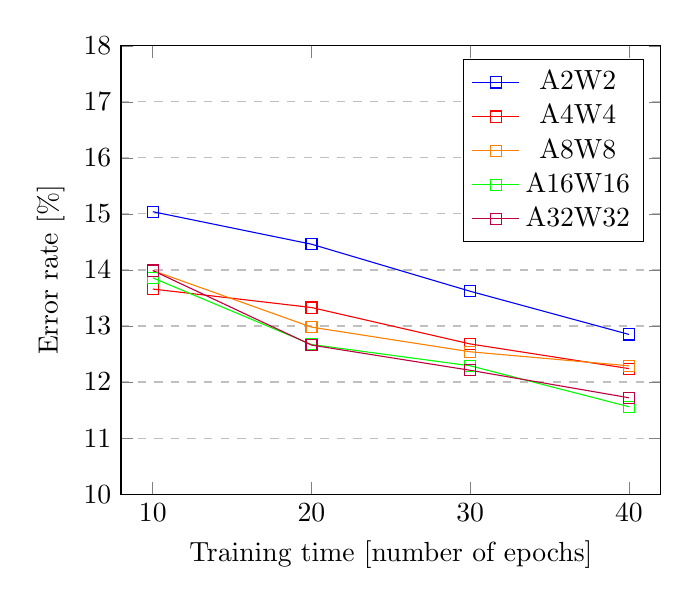
\begin{tikzpicture}
\begin{axis}[
    xlabel={Training time [number of epochs]},
    ylabel={Error rate [\%]},
    xmin=8, xmax=42,
    ymin=10, ymax=18,
    xtick={0,10,20,30,40},
    ytick={10,11,12,13,14,15,16,17,18},
    legend pos=north east,
    ymajorgrids=true,
    grid style=dashed,
]
% TFC A2W2:   84.960 | 85.540 | 86.380 | 87.150
\addplot[
    color=blue,
    mark=square,
    ]
    coordinates {
    (10,15.04)(20,14.46)(30,13.62)(40,12.85)
    };
% TFC A4W4:   86.340 | 86.670 | 87.320 | 87.760
\addplot[
    color=red,
    mark=square,
    ]
    coordinates {
    (10,13.66)(20,13.33)(30,12.68)(40,12.24)
    };
% TFC A8W8:   86.010 | 87.020 | 87.460 | 87.710
\addplot[
    color=orange,
    mark=square,
    ]
    coordinates {
    (10,13.99)(20,12.98)(30,12.54)(40,12.29)
    };
% TFC A16W16: 86.140 | 87.330 | 87.710 | 88.440
\addplot[
    color=green,
    mark=square,
    ]
    coordinates {
    (10,13.86)(20,12.67)(30,12.29)(40,11.56)
    };
% TFC A32W32: 86.010 | 87.340 | 87.690 | 88.280
\addplot[
    color=purple,
    mark=square,
    ]
    coordinates {
    (10,13.99)(20,12.66)(30,12.21)(40,11.72)
    };
\legend{A2W2,A4W4,A8W8,A16W16,A32W32}
\end{axis}
\end{tikzpicture}
\caption[TFC Error Rate]{TFC error rate against training time}
  \label{fig:TFCErrorRate}
\end{figure}

While the \emph{CNV} network could not be deployed, it could still be trained and the results can be seen on \emph{Figure} \ref{fig:CNVErrorRate}. As in the \emph{TNC} figure, the configurations are named A\emph{X}W\emph{X}, where \emph{X} is the bitwidth.

% GRAPH ACCURACY TRAINING TIME CNV
\begin{figure}[htbp]
\centering
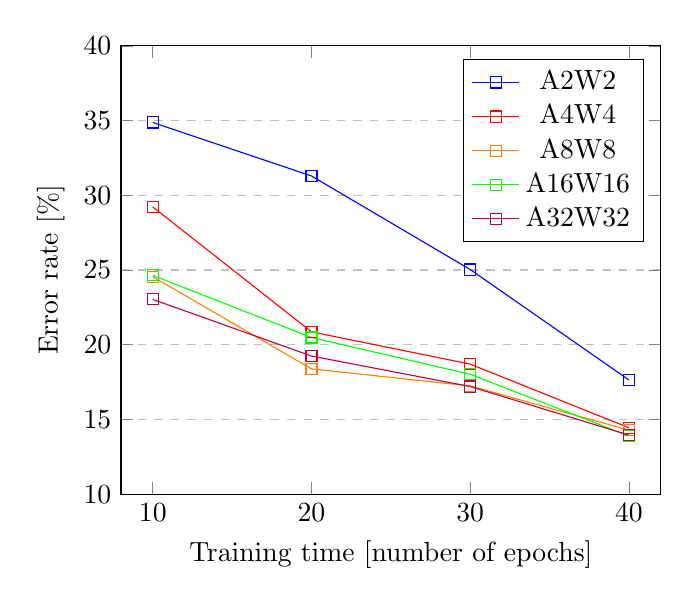
\begin{tikzpicture}
\begin{axis}[
    xlabel={Training time [number of epochs]},
    ylabel={Error rate [\%]},
    xmin=8, xmax=42,
    ymin=10, ymax=40,
    xtick={0,10,20,30,40},
    ytick={10,15,20,25,30,35,40},
    legend pos=north east,
    ymajorgrids=true,
    grid style=dashed,
]
% CNV A2W2:   65.130 | 68.710 | 76.970 | 82.360
\addplot[
    color=blue,
    mark=square,
    ]
    coordinates {
    (10,34.87)(20,31.29)(30,25.03)(40,17.64)
    };
% CNV A4W4:   70.780 | 79.140 | 81.300 | 85.560
\addplot[
    color=red,
    mark=square,
    ]
    coordinates {
    (10,29.22)(20,20.86)(30,18.70)(40,14.44)
    };
% CNV A8W8: 75.450 | 81.620 | 82.760 | 85.720
\addplot[
    color=orange,
    mark=square,
    ]
    coordinates {
    (10,24.55)(20,18.38)(30,17.24)(40,14.28)
    };
% CNV A16W16: 75.360 | 79.520 | 81.980 | 86.110
\addplot[
    color=green,
    mark=square,
    ]
    coordinates {
    (10,24.64)(20,20.48)(30,18.02)(40,13.89)
    };
% CNV A32W32: 72.970 | 80.760 | 82.800 | 86.050
\addplot[
    color=purple,
    mark=square,
    ]
    coordinates {
    (10,23.03)(20,19.24)(30,17.20)(40,13.95)
    };

\legend{A2W2,A4W4,A8W8,A16W16,A32W32}
\end{axis}
\end{tikzpicture}
\caption[CNV Error Rate]{CNV error rate against training time}
  \label{fig:CNVErrorRate}
\end{figure}

Both graphs show a separation in three sections: 2-bits precision, 4- and 8-bits precision and 16- and 32-bits precision. This separation is seen in terms of reaction to the training. For the \emph{TFC} network, the result of the training, after 40 epochs shows three separate points: $\sim$13\% error rate for A2W2, $\sim$12.3\% error rate for A4W4 and A8W8 and $\sim$11.6\% for A16E16 and A32W32. On the other hand for the \emph{CNV} network, there is a clear separation between A2W2 at $\sim$17.5\% and all the other configurations at $\sim$14.8%

Now if we look deeper into the \emph{TFC} deployment, we can get other important metrics from the experiments. First, \emph{Figure} \ref{fig:TFCThroughput} shows the throughput compared to the error rate determined earlier. Note that the error rate for a 40-epochs long training is used.

The three metrics presented in the next graphs are: \emph{throughput}, the number of images the deployed network can process in one second ; \emph{DRAM in bandwidth}, the amount of data that can be processed coming from the DRAM in to the FPGA board ; \emph{DRAM out banwidth}, the amount of data that can be processed coming from the FPGA board out to the DRAM.

\begin{itemize}
  \item \textbf{Throughput}(\emph{Figure} \ref{fig:TFCThroughput}): If the throughput seems nearly identical for A2W2 and A4W4, going to A8W8 makes one lose more than 10 thousands images per second. And even worse, using A16W16 consists of a loss of over 45 thousands images per second.

  % THROUGHPUT FIGURE
  \begin{figure}[htbp]
  \centering
  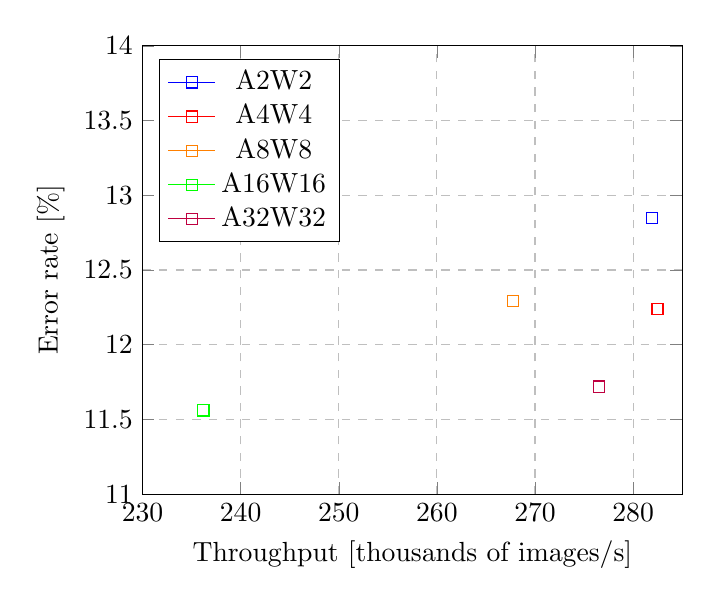
\begin{tikzpicture}
  \begin{axis}[
    xlabel={Throughput [thousands of images/s]},
    ylabel={Error rate [\%]},
    xmin=230, xmax=285,
    ymin=11, ymax=14,
    xtick={230,240,250,260,270,280},
    ytick={11,11.5,12,12.5,13,13.5,14},
    legend pos=north west,
    ymajorgrids=true,
    xmajorgrids=true,
    grid style=dashed,
    ]
  % A2W2
  \addplot+ [
      color=blue,
      mark=square
      ] coordinates {(281.951,12.85)};
  % A4W4
  \addplot+ [
      color=red,
      mark=square
      ] coordinates {(282.483,12.24)};
  % A8W8
  \addplot+ [
      color=orange,
      mark=square
      ] coordinates {(267.732,12.29)};
  % A16W16
  \addplot+ [
      color=green,
      mark=square
      ] coordinates {(236.205,11.56)};
  % A32W32
  \addplot+ [
      color=purple,
      mark=square
      ] coordinates {(276.541,11.72)};
  \legend{A2W2,A4W4,A8W8,A16W16,A32W32}
  \end{axis}
  \end{tikzpicture}
  \caption[TFC Throughput]{TFC error rate compared to throughput}
    \label{fig:TFCThroughput}
  \end{figure}


  \item \textbf{DRAM in bandwidth}(\emph{Figure} \ref{fig:TFCDRAMIn}): The same conclusions can be used for the DRAM bandwidth. The more the bitwidth, the lower the bandwidth, with an exception fo A4W4 that outperforms A2W2 being at 288 against 283 Mb/s.

  % DRAM in bandwidth FIGURE
  \begin{figure}[htbp]
  \centering
  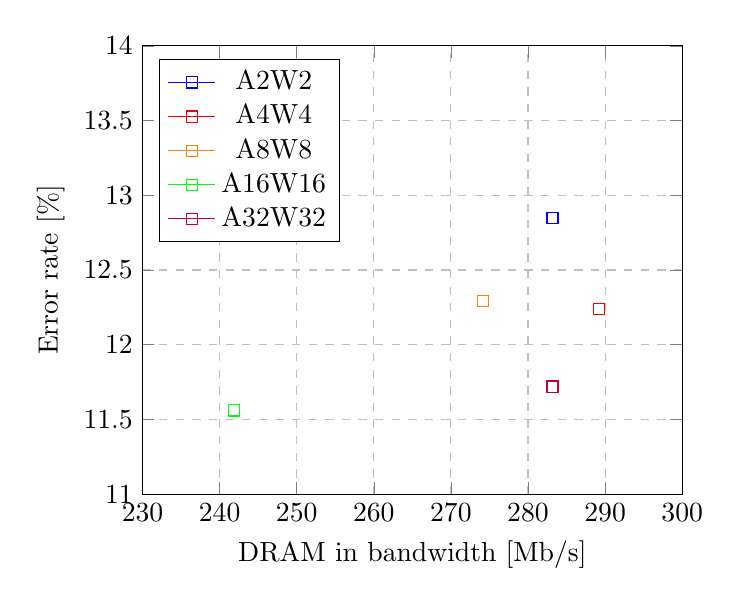
\begin{tikzpicture}
  \begin{axis}[
    xlabel={DRAM in bandwidth [Mb/s]},
    ylabel={Error rate [\%]},
    xmin=230, xmax=300,
    ymin=11, ymax=14,
    xtick={230,240,250,260,270,280,290,300},
    ytick={11,11.5,12,12.5,13,13.5,14},
    legend pos=north west,
    ymajorgrids=true,
    xmajorgrids=true,
    grid style=dashed,
    ]
  % A2W2
  \addplot+ [
      color=blue,
      mark=square
      ] coordinates {(283.18,12.85)};
  % A4W4
  \addplot+ [
      color=red,
      mark=square
      ] coordinates {(289.26,12.24)};
  % A8W8
  \addplot+ [
      color=orange,
      mark=square
      ] coordinates {(274.16,12.29)};
  % A16W16
  \addplot+ [
      color=green,
      mark=square
      ] coordinates {(241.87,11.56)};
  % A32W32
  \addplot+ [
      color=purple,
      mark=square
      ] coordinates {(283.18,11.72)};
  \legend{A2W2,A4W4,A8W8,A16W16,A32W32}
  \end{axis}
  \end{tikzpicture}
  \caption[TFC DRAM in]{TFC DRAM in bandwidth when compared to error rate}
    \label{fig:TFCDRAMIn}
  \end{figure}

  \item \textbf{DRAM out bandwidth}(\emph{Figure} \ref{fig:TFCDRAMOut}): While the graph presents the same impressions as the DRAM in, the results for A2W2 and A4W4 are this time nearly identical around 11.3Mb/s


  % DRAM out bandwidth FIGURE
  \begin{figure}[htbp]
  \centering
  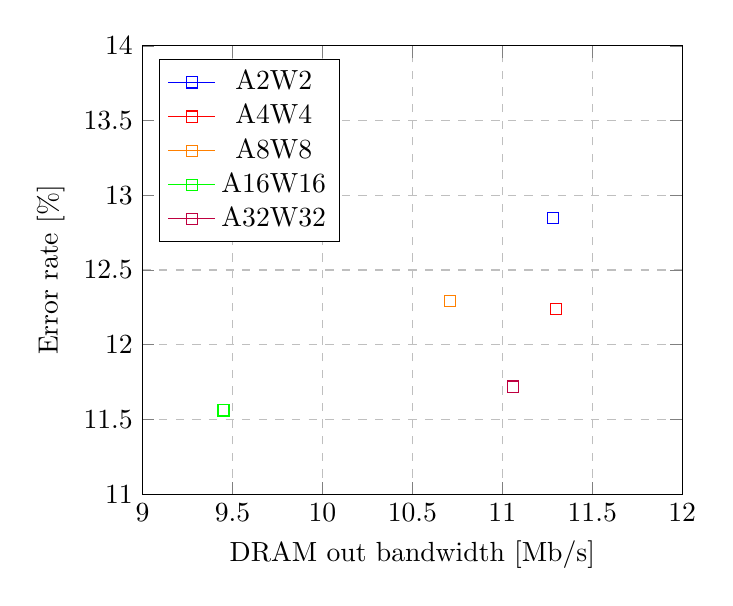
\begin{tikzpicture}
  \begin{axis}[
    xlabel={DRAM out bandwidth [Mb/s]},
    ylabel={Error rate [\%]},
    xmin=9, xmax=12,
    ymin=11, ymax=14,
    xtick={9,9.5,10,10.5,11,11.5,12},
    ytick={11,11.5,12,12.5,13,13.5,14},
    legend pos=north west,
    ymajorgrids=true,
    xmajorgrids=true,
    grid style=dashed,
    ]
  % A2W2
  \addplot+ [
      color=blue,
      mark=square
      ] coordinates {(11.28,12.85)};
  % A4W4
  \addplot+ [
      color=red,
      mark=square
      ] coordinates {(11.30,12.24)};
  % A8W8
  \addplot+ [
      color=orange,
      mark=square
      ] coordinates {(10.71,12.29)};
  % A16W16
  \addplot+ [
      color=green,
      mark=square
      ] coordinates {(9.45,11.56)};
  % A32W32
  \addplot+ [
      color=purple,
      mark=square
      ] coordinates {(11.06,11.72)};
  \legend{A2W2,A4W4,A8W8,A16W16,A32W32}
  \end{axis}
  \end{tikzpicture}
  \caption[TFC DRAM out]{TFC DRAM out bandwidth when compared to error rate}
    \label{fig:TFCDRAMOut}
  \end{figure}
\end{itemize}

%----------------------------------------------------------------------------------------
%	SUBSECTION 7.1.2 - Results Tables
%----------------------------------------------------------------------------------------

\subsection{Results Tables}

This section presents the data used to plot the different graphs from earlier but
% \begin{table}[!]
%   \centering
%   \resizebox{\textwidth}{!}{
%   \begin{tabular}{ | c | c | c | c | c | }
%     \hline
%     \textbf{Experiment Name} & \textbf{Year} &    \textbf{Paper}     & \textbf{Number of Parameters} & \textbf{Top-1 Accuracy} \\
%     \hline
%     \textbf{A2W2I8}          &     1998      &  \cite{LeCun1998}     &         0.6 M                 &           X             \\
%     \hline
%     \textbf{A4W4I8}          &     2012      & \cite{Krizhevsky2012} &          60 M                 &         63.3\%          \\
%     \hline
%     \textbf{A8W8I8}          &     2014      & \cite{Simonyan2014}   &         138 M                 &         74.4\%          \\
%     \hline
%     \textbf{A16W16I32}       &     2015      & \cite{He2015}         &          26 M                 &         81.2\%          \\
%     \hline
%     \textbf{A32W32I32}       &     2017      & \cite{Howard2017}     &         4.2 M                 &         72.56\%         \\
%     \hline
%   \end{tabular}
%   }
% \caption[Zebi]{Convolutional Neural Network Architectures}
% \label{tab:Zebi}
% \end{table}


% TFC
% Results for            Throughput | DRAM in bandwidth | DRAM out bandwidth:
% A2W2:   281951 (img/s) | 283.18 (Mb/s)     | 11.28  (Mb/s)
% A4W4:   282483 (img/s) | 289.26 (Mb/s)     | 11.30  (Mb/s)
% A8W8:   267732 (img/s) | 274.16 (Mb/s)     | 10.71  (Mb/s)
% A16W16: 236205 (img/s) | 241.87 (Mb/s)     | 9.45   (Mb/s)
% A32W32: 276541 (img/s) | 283.18 (Mb/s)     | 11.06  (MB/s)
%
% TFC
% Results for Accuracy 10 | 20 | 30 | 40 epochs
% A2W2:   84.960 | 85.540 | 86.380 | 87.150
% A4W4:   86.340 | 86.670 | 87.320 | 87.760
% A8W8:   86.010 | 87.020 | 87.460 | 87.710
% A16W16: 86.140 | 87.330 | 87.710 | 88.440
% A32W32: 86.010 | 87.340 | 87.690 | 88.280
%
% CNV
% Results for Accuracy 10 | 20 | 30 | 40 epochs
% A2W2:   65.130 | 68.710 | 76.970 | 82.360
% A4W4:   70.780 | 79.140 | 81.300 | 85.560
% A8W8:   75.450 | 81.620 | 82.760 | 85.720
% A16W16: 75.360 | 79.520 | 81.980 | 86.110
% A32W32: 72.970 | 80.760 | 82.800 | 86.050

%----------------------------------------------------------------------------------------
%	SUBSECTION 7.1.3 - Results Conclusion
%----------------------------------------------------------------------------------------

\subsection{Results Conclusion}

\chapter{Discussion \& Evaluation} % Main chapter title

\label{Chapter8} % For referencing this chapter elsewhere, use \ref{Chapter9}

\lhead{Chapter 8. \emph{Discussion \& Evaluation}}

%----------------------------------------------------------------------------------------
%	SECTION 8.1 - Discussion
%----------------------------------------------------------------------------------------

\section{Discussion}

%----------------------------------------------------------------------------------------
%	SECTION 8.2.1 - Network Architectures
%----------------------------------------------------------------------------------------

\subsection{Network Architectures}

The chosen architectures used during the experiments

%----------------------------------------------------------------------------------------
%	SECTION 8.2.2 - Datasets
%----------------------------------------------------------------------------------------

\subsection{Datasets}

Datasets taken


%----------------------------------------------------------------------------------------
%	SECTION 8.2.3 - Training Process
%----------------------------------------------------------------------------------------

\subsection{Training Process}

Training process was taken from ref? To be extended to compare if higher precision for less long is better than lower precision for a longer time.

%----------------------------------------------------------------------------------------
%	SECTION 8.2.4 - Deployment Process
%----------------------------------------------------------------------------------------

\subsection{Deployment Process}

The deployment process depends on two main points: Transformations used and Folding proposed.

%----------------------------------------------------------------------------------------
%	SECTION 8.2.5 - Weight and Activation Bitwidths
%----------------------------------------------------------------------------------------

\subsection{Weight and Activation Bitwidths}

The activation bitwidth used were taken specifically

%----------------------------------------------------------------------------------------
%	SECTION 8.3 - Evaluation
%----------------------------------------------------------------------------------------

\section{Evaluation}

%----------------------------------------------------------------------------------------
%	SUBSECTION 8.3.1 - Comparison to the literature
%----------------------------------------------------------------------------------------

\subsection{Comparison to the literature}

Comparison \emph{TFC} / \emph{Fashion-MNIST} with other results from the literature.

Comparison \emph{CNV} / \emph{CIFAR-10} with other results from the literature.
%----------------------------------------------------------------------------------------
%	SUBSECTION 8.3.2 - Future Works
%----------------------------------------------------------------------------------------

\subsection{Future Works}

Limits presented in the discussion section.

\chapter{Conclusion} % Main chapter title

\label{Chapter9} % For referencing this chapter elsewhere, use \ref{Chapter9}

\lhead{Chapter 9. \emph{Conclusion}}

The objectives of the given document are to extend the earlier \emph{Research Report} that was covering the background and literature review. The background of the project consists of three main axis. First, the importance of \emph{number representation} and the underlying trade-offs it implies both in terms of power consumptions and memory space. Then, the mechanics of \emph{machine learning} when applied to image classification through renowned architectures and datasets to finally highlight the potential mixed-precision vectors. Finally, the importance of the choice of the \emph{hardware architecture} is presented and FPGA are shown to be an interesting in-between for efficiency and flexibility. In the literature review part, \emph{mixed-precision} is presented then applied to neural network with \emph{quantisation} and deployed to FPGAs with \emph{frameworks}. While the literature review had to be reworked to be recentred here, the chosen project remained the same: the development of a benchmark for quantised neural networks to be deployed on reconfigurable architectures. Several frameworks propose this deployment but few are still in active development or open-source. \emph{FINN} and the network trainer \emph{Brevitas} propose a path to design, train and deploy a quantised neural network on an FPGA board.

The development of a benchmark on top of the \emph{Brevitas} / \emph{FINN} workflow helped to assess the impact of mixed-precision on deployed quantised neural networks. The results present an intuitive relation for configurations using 2-bits precision up to 16-bits precision. The difference in end accuracy when comparing the two is manageable and consists of less than one percent. However, a considerable gain is noticeable in throughput and DRAM bandwidth. Now the results highlighted other more unsettling results. First, the representation using 32-bits precisions outperforms several others in terms of throughput and bandwidth and gathers scores similar to 2 or 4 bits representations. Following the same path, the hardware utilisation of the different configurations is extremely similar. Few differences in terms of LUTs, FFs or BRAMs can be noticed.

While these results are counter-intuitive to some extent, they highlight the need to benchmark more the different quantisation frameworks, whether they are for classic applications (Distiller, PyTorch or TensorFlow extensions, etc.) or specifically revolving around FPGA deployment. The results have been transmitted to the Xilinx Research Team working on the \emph{FINN} / \emph{Brevitas} workflow. They want to investigate the different issues of both the performance of the 32-bits configuration and very similar hardware utilisations between the different configurations.

Future works can be conducted following thee axis. First, the extension of the present benchmark to renowned architectures and datasets. This step will require to wait or participate in the development of the framework as several network configurations are not supported for now. Second, the extension of this benchmark to other frameworks that perform similar actions to deploy neural networks on FPGAs or simply compare the training accuracies with more classic implementations. Finally, as \cite{Bacchus2020} performed, assess the importance of the bit-width of weights and activations separately would help determine a sweet spot for those.


%----------------------------------------------------------------------------------------
%	THESIS CONTENT - APPENDICES
%----------------------------------------------------------------------------------------

\addtocontents{toc}{\vspace{2em}} % Add a gap in the Contents, for aesthetics

\appendix % Cue to tell LaTeX that the following 'chapters' are Appendices

% Include the appendices of the thesis as separate files from the Appendices folder
% Uncomment the lines as you write the Appendices

% Appendix A

\chapter{Hardware Utilisation Results} % Main appendix title

\label{AppendixA} % For referencing this appendix elsewhere, use \ref{AppendixA}

\lhead{Appendix A. \emph{Hardware Utilisation Results}} % This is for the header on each page - perhaps a shortened title

This appendix contains the detailed results of the hardware utilisation for the different configuration. In the tables can be found the total number of resources used under the \texttt{resizer\_wrapper}, the used resources for the important \emph{IP}s of the system following and the different layers that begin with \texttt{Streaming...}.



\begin{landscape}

\begin{table}[!htb]
\resizebox{24cm}{!}{
\begin{tabular}{l|l|l|l|l|l|l|l|l|l|l}
   \textbf{Instance}                                         & \textbf{Module}                                                                                        & \textbf{Total LUTs} & \textbf{Logic LUTs} & \textbf{LUTRAMs} & \textbf{SRLs} & \textbf{FFs}   & \textbf{RAMB36} & \textbf{RAMB18} & \textbf{DSP48 Blocks} \\
   resizer\_wrapper                                        & (top)                                                                                                  & 31622      & 28324      & 1302    & 1996 & 27989 & 40     & 3      & 0            \\
   resizer\_i                                              & resizer                                                                                                & 31622      & 28324      & 1302    & 1996 & 27989 & 40     & 3      & 0            \\
   axi\_dma\_0                                             & resizer\_axi\_dma\_0\_0                                                                                & 1960       & 1750       & 12      & 198  & 2626  & 8      & 2      & 0            \\
   axi\_interconnect\_0                                    & resizer\_axi\_interconnect\_0\_0                                                                       & 551        & 486        & 0       & 65   & 694   & 0      & 0      & 0            \\
   axi\_protocol\_convert\_0                               & resizer\_axi\_protocol\_convert\_0\_0                                                                  & 393        & 383        & 10      & 0    & 430   & 0      & 0      & 0            \\
   axis\_dwidth\_converter\_0                              & resizer\_axis\_dwidth\_converter\_0\_0                                                                 & 21         & 21         & 0       & 0    & 370   & 0      & 0      & 0            \\
   axis\_dwidth\_converter\_1                              & resizer\_axis\_dwidth\_converter\_1\_0                                                                 & 335        & 335        & 0       & 0    & 995   & 0      & 0      & 0            \\
   processing\_system7\_0                                  & resizer\_processing\_system7\_0\_0                                                                     & 112        & 112        & 0       & 0    & 0     & 0      & 0      & 0            \\
   resize\_accel\_0                                        & resizer\_resize\_accel\_0\_0                                                                           & 28231      & 25219      & 1280    & 1732 & 22834 & 32     & 1      & 0            \\
   rst\_ps7\_0\_100M                                       & resizer\_rst\_ps7\_0\_100M\_0                                                                          & 19         & 18         & 0       & 1    & 40    & 0      & 0      & 0            \\
   StreamingDataWidthConverter\_Batch\_0                   & resizer\_resize\_accel\_0\_0\_finn\_design\_StreamingDataWidthConverter\_Batch\_0\_0                   & 101        & 101        & 0       & 0    & 196   & 0      & 0      & 0            \\
   StreamingFCLayer\_Batch\_0                              & resizer\_resize\_accel\_0\_0\_finn\_design\_StreamingFCLayer\_Batch\_0\_0                              & 19464      & 18439      & 0       & 1025 & 16314 & 28     & 1      & 0            \\
   StreamingFCLayer\_Batch\_1                              & resizer\_resize\_accel\_0\_0\_finn\_design\_StreamingFCLayer\_Batch\_1\_0                              & 2254       & 2189       & 0       & 65   & 1634  & 2      & 0      & 0            \\
   StreamingFCLayer\_Batch\_2                              & resizer\_resize\_accel\_0\_0\_finn\_design\_StreamingFCLayer\_Batch\_2\_0                              & 2260       & 2195       & 0       & 65   & 1640  & 2      & 0      & 0            \\
   StreamingFCLayer\_Batch\_3                              & resizer\_resize\_accel\_0\_0\_finn\_design\_StreamingFCLayer\_Batch\_3\_0                              & 2472       & 1111       & 1280    & 81   & 1491  & 0      & 0      & 0            \\
   StreamingFIFO\_0                                        & resizer\_resize\_accel\_0\_0\_finn\_design\_StreamingFIFO\_0\_0                                        & 542        & 286        & 0       & 256  & 276   & 0      & 0      & 0            \\
   StreamingFIFO\_1                                        & resizer\_resize\_accel\_0\_0\_finn\_design\_StreamingFIFO\_1\_0                                        & 91         & 59         & 0       & 32   & 42    & 0      & 0      & 0            \\
   StreamingFIFO\_2                                        & resizer\_resize\_accel\_0\_0\_finn\_design\_StreamingFIFO\_2\_0                                        & 59         & 43         & 0       & 16   & 26    & 0      & 0      & 0            \\
   StreamingFIFO\_3                                        & resizer\_resize\_accel\_0\_0\_finn\_design\_StreamingFIFO\_3\_0                                        & 59         & 43         & 0       & 16   & 26    & 0      & 0      & 0            \\
   StreamingFIFO\_4                                        & resizer\_resize\_accel\_0\_0\_finn\_design\_StreamingFIFO\_4\_0                                        & 59         & 43         & 0       & 16   & 26    & 0      & 0      & 0            \\
   StreamingFIFO\_5                                        & resizer\_resize\_accel\_0\_0\_finn\_design\_StreamingFIFO\_5\_0                                        & 338        & 178        & 0       & 160  & 169   & 0      & 0      & 0            \\
   TLastMarker\_0                                          & resizer\_resize\_accel\_0\_0\_finn\_design\_TLastMarker\_0\_0                                          & 532        & 532        & 0       & 0    & 994   & 0      & 0      & 0            \\
\end{tabular}
}
\caption[TFC Hardware Utilisation A2W2]{TFC Hardware Utilisation for A2W2 configuration}
  \label{tab:TFCHardwareA2W2}
\end{table}


\begin{table}[!htb]
\resizebox{24cm}{!}{
\begin{tabular}{l|l|l|l|l|l|l|l|l|l|l}
   \textbf{Instance}                                         & \textbf{Module}                                                                                        & \textbf{Total LUTs} & \textbf{Logic LUTs} & \textbf{LUTRAMs} & \textbf{SRLs} & \textbf{FFs}   & \textbf{RAMB36} & \textbf{RAMB18} & \textbf{DSP48 Blocks} \\
   resizer\_wrapper                                        & (top)                                                                                                  & 31614      & 28316      & 1302    & 1996 & 28052 & 40     & 3      & 0            \\
   resizer\_i                                              & resizer                                                                                                & 31614      & 28316      & 1302    & 1996 & 28052 & 40     & 3      & 0            \\
   axi\_dma\_0                                             & resizer\_axi\_dma\_0\_0                                                                                & 1960       & 1750       & 12      & 198  & 2626  & 8      & 2      & 0            \\
   axi\_interconnect\_0                                    & resizer\_axi\_interconnect\_0\_0                                                                       & 551        & 486        & 0       & 65   & 694   & 0      & 0      & 0            \\
   axi\_protocol\_convert\_0                               & resizer\_axi\_protocol\_convert\_0\_0                                                                  & 393        & 383        & 10      & 0    & 430   & 0      & 0      & 0            \\
   axis\_dwidth\_converter\_0                              & resizer\_axis\_dwidth\_converter\_0\_0                                                                 & 21         & 21         & 0       & 0    & 370   & 0      & 0      & 0            \\
   axis\_dwidth\_converter\_1                              & resizer\_axis\_dwidth\_converter\_1\_0                                                                 & 335        & 335        & 0       & 0    & 995   & 0      & 0      & 0            \\
   processing\_system7\_0                                  & resizer\_processing\_system7\_0\_0                                                                     & 112        & 112        & 0       & 0    & 0     & 0      & 0      & 0            \\
   resize\_accel\_0                                        & resizer\_resize\_accel\_0\_0                                                                           & 28223      & 25211      & 1280    & 1732 & 22897 & 32     & 1      & 0            \\
   rst\_ps7\_0\_100M                                       & resizer\_rst\_ps7\_0\_100M\_0                                                                          & 19         & 18         & 0       & 1    & 40    & 0      & 0      & 0            \\
   StreamingDataWidthConverter\_Batch\_0                   & resizer\_resize\_accel\_0\_0\_finn\_design\_StreamingDataWidthConverter\_Batch\_0\_0                   & 101        & 101        & 0       & 0    & 196   & 0      & 0      & 0            \\
   StreamingFCLayer\_Batch\_0                              & resizer\_resize\_accel\_0\_0\_finn\_design\_StreamingFCLayer\_Batch\_0\_0                              & 19505      & 18480      & 0       & 1025 & 16461 & 28     & 1      & 0            \\
   StreamingFCLayer\_Batch\_1                              & resizer\_resize\_accel\_0\_0\_finn\_design\_StreamingFCLayer\_Batch\_1\_0                              & 2223       & 2158       & 0       & 65   & 1583  & 2      & 0      & 0            \\
   StreamingFCLayer\_Batch\_2                              & resizer\_resize\_accel\_0\_0\_finn\_design\_StreamingFCLayer\_Batch\_2\_0                              & 2242       & 2177       & 0       & 65   & 1607  & 2      & 0      & 0            \\
   StreamingFCLayer\_Batch\_3                              & resizer\_resize\_accel\_0\_0\_finn\_design\_StreamingFCLayer\_Batch\_3\_0                              & 2472       & 1111       & 1280    & 81   & 1491  & 0      & 0      & 0            \\
   StreamingFIFO\_0                                        & resizer\_resize\_accel\_0\_0\_finn\_design\_StreamingFIFO\_0\_0                                        & 542        & 286        & 0       & 256  & 276   & 0      & 0      & 0            \\
   StreamingFIFO\_1                                        & resizer\_resize\_accel\_0\_0\_finn\_design\_StreamingFIFO\_1\_0                                        & 91         & 59         & 0       & 32   & 42    & 0      & 0      & 0            \\
   StreamingFIFO\_2                                        & resizer\_resize\_accel\_0\_0\_finn\_design\_StreamingFIFO\_2\_0                                        & 59         & 43         & 0       & 16   & 26    & 0      & 0      & 0            \\
   StreamingFIFO\_3                                        & resizer\_resize\_accel\_0\_0\_finn\_design\_StreamingFIFO\_3\_0                                        & 59         & 43         & 0       & 16   & 26    & 0      & 0      & 0            \\
   StreamingFIFO\_4                                        & resizer\_resize\_accel\_0\_0\_finn\_design\_StreamingFIFO\_4\_0                                        & 59         & 43         & 0       & 16   & 26    & 0      & 0      & 0            \\
   StreamingFIFO\_5                                        & resizer\_resize\_accel\_0\_0\_finn\_design\_StreamingFIFO\_5\_0                                        & 338        & 178        & 0       & 160  & 169   & 0      & 0      & 0            \\
   TLastMarker\_0                                          & resizer\_resize\_accel\_0\_0\_finn\_design\_TLastMarker\_0\_0                                          & 532        & 532        & 0       & 0    & 994   & 0      & 0      & 0            \\
\end{tabular}
}
\caption[TFC Hardware Utilisation A4W4]{TFC Hardware Utilisation for A4W4 configuration}
  \label{tab:TFCHardwareA4W4}
\end{table}

\begin{table}[!htb]
\resizebox{24cm}{!}{
\begin{tabular}{l|l|l|l|l|l|l|l|l|l|l}
   \textbf{Instance}                                         & \textbf{Module}                                                                                        & \textbf{Total LUTs} & \textbf{Logic LUTs} & \textbf{LUTRAMs} & \textbf{SRLs} & \textbf{FFs}   & \textbf{RAMB36} & \textbf{RAMB18} & \textbf{DSP48 Blocks} \\
   resizer\_wrapper                                        & (top)                                                                                                & 31653      & 28355      & 1302    & 1996 & 27953 & 40     & 3      & 0            \\
   resizer\_i                                              & resizer                                                                                              & 31653      & 28355      & 1302    & 1996 & 27953 & 40     & 3      & 0            \\
   axi\_dma\_0                                             & resizer\_axi\_dma\_0\_0                                                                              & 1960       & 1750       & 12      & 198  & 2626  & 8      & 2      & 0            \\
   axi\_interconnect\_0                                    & resizer\_axi\_interconnect\_0\_0                                                                     & 551        & 486        & 0       & 65   & 694   & 0      & 0      & 0            \\
   axi\_protocol\_convert\_0                               & resizer\_axi\_protocol\_convert\_0\_0                                                                & 393        & 383        & 10      & 0    & 430   & 0      & 0      & 0            \\
   axis\_dwidth\_converter\_0                              & resizer\_axis\_dwidth\_converter\_0\_0                                                               & 21         & 21         & 0       & 0    & 370   & 0      & 0      & 0            \\
   axis\_dwidth\_converter\_1                              & resizer\_axis\_dwidth\_converter\_1\_0                                                               & 335        & 335        & 0       & 0    & 995   & 0      & 0      & 0            \\
   processing\_system7\_0                                  & resizer\_processing\_system7\_0\_0                                                                   & 112        & 112        & 0       & 0    & 0     & 0      & 0      & 0            \\
   resize\_accel\_0                                        & resizer\_resize\_accel\_0\_0                                                                         & 28262      & 25250      & 1280    & 1732 & 22798 & 32     & 1      & 0            \\
   rst\_ps7\_0\_100M                                       & resizer\_rst\_ps7\_0\_100M\_0                                                                        & 19         & 18         & 0       & 1    & 40    & 0      & 0      & 0            \\
   StreamingDataWidthConverter\_Batch\_0                   & resizer\_resize\_accel\_0\_0\_finn\_design\_StreamingDataWidthConverter\_Batch\_0\_0                 & 101        & 101        & 0       & 0    & 196   & 0      & 0      & 0            \\
   StreamingFCLayer\_Batch\_0                              & resizer\_resize\_accel\_0\_0\_finn\_design\_StreamingFCLayer\_Batch\_0\_0                            & 19568      & 18543      & 0       & 1025 & 16406 & 28     & 1      & 0            \\
   StreamingFCLayer\_Batch\_1                              & resizer\_resize\_accel\_0\_0\_finn\_design\_StreamingFCLayer\_Batch\_1\_0                            & 2217       & 2152       & 0       & 65   & 1557  & 2      & 0      & 0            \\
   StreamingFCLayer\_Batch\_2                              & resizer\_resize\_accel\_0\_0\_finn\_design\_StreamingFCLayer\_Batch\_2\_0                            & 2224       & 2159       & 0       & 65   & 1589  & 2      & 0      & 0            \\
   StreamingFCLayer\_Batch\_3                              & resizer\_resize\_accel\_0\_0\_finn\_design\_StreamingFCLayer\_Batch\_3\_0                            & 2472       & 1111       & 1280    & 81   & 1491  & 0      & 0      & 0            \\
   StreamingFIFO\_0                                        & resizer\_resize\_accel\_0\_0\_finn\_design\_StreamingFIFO\_0\_0                                      & 542        & 286        & 0       & 256  & 276   & 0      & 0      & 0            \\
   StreamingFIFO\_1                                        & resizer\_resize\_accel\_0\_0\_finn\_design\_StreamingFIFO\_1\_0                                      & 91         & 59         & 0       & 32   & 42    & 0      & 0      & 0            \\
   StreamingFIFO\_2                                        & resizer\_resize\_accel\_0\_0\_finn\_design\_StreamingFIFO\_2\_0                                      & 59         & 43         & 0       & 16   & 26    & 0      & 0      & 0            \\
   StreamingFIFO\_3                                        & resizer\_resize\_accel\_0\_0\_finn\_design\_StreamingFIFO\_3\_0                                      & 59         & 43         & 0       & 16   & 26    & 0      & 0      & 0            \\
   StreamingFIFO\_4                                        & resizer\_resize\_accel\_0\_0\_finn\_design\_StreamingFIFO\_4\_0                                      & 59         & 43         & 0       & 16   & 26    & 0      & 0      & 0            \\
   StreamingFIFO\_5                                        & resizer\_resize\_accel\_0\_0\_finn\_design\_StreamingFIFO\_5\_0                                      & 338        & 178        & 0       & 160  & 169   & 0      & 0      & 0            \\
   TLastMarker\_0                                          & resizer\_resize\_accel\_0\_0\_finn\_design\_TLastMarker\_0\_0                                        & 532        & 532        & 0       & 0    & 994   & 0      & 0      & 0            \\
\end{tabular}
}
\caption[TFC Hardware Utilisation A8W8]{TFC Hardware Utilisation for A8W8 configuration}
  \label{tab:TFCHardwareA8W8}
\end{table}

\begin{table}[!htb]
\resizebox{24cm}{!}{
\begin{tabular}{l|l|l|l|l|l|l|l|l|l|l}
   \textbf{Instance}                                         & \textbf{Module}                                                                                        & \textbf{Total LUTs} & \textbf{Logic LUTs} & \textbf{LUTRAMs} & \textbf{SRLs} & \textbf{FFs}   & \textbf{RAMB36} & \textbf{RAMB18} & \textbf{DSP48 Blocks} \\
   resizer\_wrapper                                        & (top)                                                                                                  & 31612      & 28314      & 1302    & 1996 & 27997 & 40     & 3      & 0            \\
   resizer\_i                                              & resizer                                                                                                & 31612      & 28314      & 1302    & 1996 & 27997 & 40     & 3      & 0            \\
   axi\_dma\_0                                             & resizer\_axi\_dma\_0\_0                                                                                & 1960       & 1750       & 12      & 198  & 2626  & 8      & 2      & 0            \\
   axi\_interconnect\_0                                    & resizer\_axi\_interconnect\_0\_0                                                                       & 551        & 486        & 0       & 65   & 694   & 0      & 0      & 0            \\
   axi\_protocol\_convert\_0                               & resizer\_axi\_protocol\_convert\_0\_0                                                                  & 393        & 383        & 10      & 0    & 430   & 0      & 0      & 0            \\
   axis\_dwidth\_converter\_0                              & resizer\_axis\_dwidth\_converter\_0\_0                                                                 & 21         & 21         & 0       & 0    & 370   & 0      & 0      & 0            \\
   axis\_dwidth\_converter\_1                              & resizer\_axis\_dwidth\_converter\_1\_0                                                                 & 335        & 335        & 0       & 0    & 995   & 0      & 0      & 0            \\
   processing\_system7\_0                                  & resizer\_processing\_system7\_0\_0                                                                     & 112        & 112        & 0       & 0    & 0     & 0      & 0      & 0            \\
   resize\_accel\_0                                        & resizer\_resize\_accel\_0\_0                                                                           & 28221      & 25209      & 1280    & 1732 & 22842 & 32     & 1      & 0            \\
   rst\_ps7\_0\_100M                                       & resizer\_rst\_ps7\_0\_100M\_0                                                                          & 19         & 18         & 0       & 1    & 40    & 0      & 0      & 0            \\
   StreamingDataWidthConverter\_Batch\_0                   & resizer\_resize\_accel\_0\_0\_finn\_design\_StreamingDataWidthConverter\_Batch\_0\_0                   & 101        & 101        & 0       & 0    & 196   & 0      & 0      & 0            \\
   StreamingFCLayer\_Batch\_0                              & resizer\_resize\_accel\_0\_0\_finn\_design\_StreamingFCLayer\_Batch\_0\_0                              & 19521      & 18496      & 0       & 1025 & 16462 & 28     & 1      & 0            \\
   StreamingFCLayer\_Batch\_1                              & resizer\_resize\_accel\_0\_0\_finn\_design\_StreamingFCLayer\_Batch\_1\_0                              & 2218       & 2153       & 0       & 65   & 1559  & 2      & 0      & 0            \\
   StreamingFCLayer\_Batch\_2                              & resizer\_resize\_accel\_0\_0\_finn\_design\_StreamingFCLayer\_Batch\_2\_0                              & 2229       & 2164       & 0       & 65   & 1575  & 2      & 0      & 0            \\
   StreamingFCLayer\_Batch\_3                              & resizer\_resize\_accel\_0\_0\_finn\_design\_StreamingFCLayer\_Batch\_3\_0                              & 2472       & 1111       & 1280    & 81   & 1491  & 0      & 0      & 0            \\
   StreamingFIFO\_0                                        & resizer\_resize\_accel\_0\_0\_finn\_design\_StreamingFIFO\_0\_0                                        & 542        & 286        & 0       & 256  & 276   & 0      & 0      & 0            \\
   StreamingFIFO\_1                                        & resizer\_resize\_accel\_0\_0\_finn\_design\_StreamingFIFO\_1\_0                                        & 91         & 59         & 0       & 32   & 42    & 0      & 0      & 0            \\
   StreamingFIFO\_2                                        & resizer\_resize\_accel\_0\_0\_finn\_design\_StreamingFIFO\_2\_0                                        & 59         & 43         & 0       & 16   & 26    & 0      & 0      & 0            \\
   StreamingFIFO\_3                                        & resizer\_resize\_accel\_0\_0\_finn\_design\_StreamingFIFO\_3\_0                                        & 59         & 43         & 0       & 16   & 26    & 0      & 0      & 0            \\
   StreamingFIFO\_4                                        & resizer\_resize\_accel\_0\_0\_finn\_design\_StreamingFIFO\_4\_0                                        & 59         & 43         & 0       & 16   & 26    & 0      & 0      & 0            \\
   TLastMarker\_0                                          & resizer\_resize\_accel\_0\_0\_finn\_design\_TLastMarker\_0\_0                                          & 532        & 532        & 0       & 0    & 994   & 0      & 0      & 0            \\
\end{tabular}
}
\caption[TFC Hardware Utilisation A16W16]{TFC Hardware Utilisation for A16W16 configuration}
  \label{tab:TFCHardwareA16W16}
\end{table}


\begin{table}[!htb]
\resizebox{24cm}{!}{
\begin{tabular}{l|l|l|l|l|l|l|l|l|l|l}
   \textbf{Instance}                                         & \textbf{Module}                                                                                        & \textbf{Total LUTs} & \textbf{Logic LUTs} & \textbf{LUTRAMs} & \textbf{SRLs} & \textbf{FFs}   & \textbf{RAMB36} & \textbf{RAMB18} & \textbf{DSP48 Blocks} \\
   resizer\_wrapper                                        & (top)                                                                                                  & 31599      & 28301      & 1302    & 1996 & 27949 & 40     & 3      & 0            \\
   resizer\_i                                              & resizer                                                                                                & 31599      & 28301      & 1302    & 1996 & 27949 & 40     & 3      & 0            \\
   axi\_dma\_0                                             & resizer\_axi\_dma\_0\_0                                                                                & 1960       & 1750       & 12      & 198  & 2626  & 8      & 2      & 0            \\
   axi\_interconnect\_0                                    & resizer\_axi\_interconnect\_0\_0                                                                       & 551        & 486        & 0       & 65   & 694   & 0      & 0      & 0            \\
   axi\_protocol\_convert\_0                               & resizer\_axi\_protocol\_convert\_0\_0                                                                  & 393        & 383        & 10      & 0    & 430   & 0      & 0      & 0            \\
   axis\_dwidth\_converter\_0                              & resizer\_axis\_dwidth\_converter\_0\_0                                                                 & 21         & 21         & 0       & 0    & 370   & 0      & 0      & 0            \\
   axis\_dwidth\_converter\_1                              & resizer\_axis\_dwidth\_converter\_1\_0                                                                 & 335        & 335        & 0       & 0    & 995   & 0      & 0      & 0            \\
   processing\_system7\_0                                  & resizer\_processing\_system7\_0\_0                                                                     & 112        & 112        & 0       & 0    & 0     & 0      & 0      & 0            \\
   resize\_accel\_0                                        & resizer\_resize\_accel\_0\_0                                                                           & 28208      & 25196      & 1280    & 1732 & 22794 & 32     & 1      & 0            \\
   rst\_ps7\_0\_100M                                       & resizer\_rst\_ps7\_0\_100M\_0                                                                          & 19         & 18         & 0       & 1    & 40    & 0      & 0      & 0            \\
   StreamingDataWidthConverter\_Batch\_0                   & resizer\_resize\_accel\_0\_0\_finn\_design\_StreamingDataWidthConverter\_Batch\_0\_0                   & 101        & 101        & 0       & 0    & 196   & 0      & 0      & 0            \\
   StreamingFCLayer\_Batch\_0                              & resizer\_resize\_accel\_0\_0\_finn\_design\_StreamingFCLayer\_Batch\_0\_0                              & 19511      & 18486      & 0       & 1025 & 16414 & 28     & 1      & 0            \\
   StreamingFCLayer\_Batch\_1                              & resizer\_resize\_accel\_0\_0\_finn\_design\_StreamingFCLayer\_Batch\_1\_0                              & 2217       & 2152       & 0       & 65   & 1554  & 2      & 0      & 0            \\
   StreamingFCLayer\_Batch\_2                              & resizer\_resize\_accel\_0\_0\_finn\_design\_StreamingFCLayer\_Batch\_2\_0                              & 2227       & 2162       & 0       & 65   & 1580  & 2      & 0      & 0            \\
   StreamingFCLayer\_Batch\_3                              & resizer\_resize\_accel\_0\_0\_finn\_design\_StreamingFCLayer\_Batch\_3\_0                              & 2472       & 1111       & 1280    & 81   & 1491  & 0      & 0      & 0            \\
   StreamingFIFO\_0                                        & resizer\_resize\_accel\_0\_0\_finn\_design\_StreamingFIFO\_0\_0                                        & 542        & 286        & 0       & 256  & 276   & 0      & 0      & 0            \\
   StreamingFIFO\_1                                        & resizer\_resize\_accel\_0\_0\_finn\_design\_StreamingFIFO\_1\_0                                        & 91         & 59         & 0       & 32   & 42    & 0      & 0      & 0            \\
   StreamingFIFO\_2                                        & resizer\_resize\_accel\_0\_0\_finn\_design\_StreamingFIFO\_2\_0                                        & 59         & 43         & 0       & 16   & 26    & 0      & 0      & 0            \\
   StreamingFIFO\_3                                        & resizer\_resize\_accel\_0\_0\_finn\_design\_StreamingFIFO\_3\_0                                        & 59         & 43         & 0       & 16   & 26    & 0      & 0      & 0            \\
   StreamingFIFO\_4                                        & resizer\_resize\_accel\_0\_0\_finn\_design\_StreamingFIFO\_4\_0                                        & 59         & 43         & 0       & 16   & 26    & 0      & 0      & 0            \\
   StreamingFIFO\_5                                        & resizer\_resize\_accel\_0\_0\_finn\_design\_StreamingFIFO\_5\_0                                        & 338        & 178        & 0       & 160  & 169   & 0      & 0      & 0            \\
   TLastMarker\_0                                          & resizer\_resize\_accel\_0\_0\_finn\_design\_TLastMarker\_0\_0                                          & 532        & 532        & 0       & 0    & 994   & 0      & 0      & 0            \\
\end{tabular}
}
\caption[TFC Hardware Utilisation A32W32]{TFC Hardware Utilisation for A32W32 configuration}
  \label{tab:TFCHardwareA32W32}
\end{table}

\end{landscape}

%\input{Appendices/AppendixB}
%\input{Appendices/AppendixC}

\addtocontents{toc}{\vspace{2em}} % Add a gap in the Contents, for aesthetics

\backmatter

%----------------------------------------------------------------------------------------
%	BIBLIOGRAPHY
%----------------------------------------------------------------------------------------

\label{Bibliography}

\lhead{\emph{Bibliography}} % Change the page header to say "Bibliography"

\bibliographystyle{IEEEtran} % Biblio style can be changed !

\bibliography{Bibliography} % The references (bibliography) information are stored in the file named "Bibliography.bib"

\end{document}
